\documentclass[12pt,a4paper]{article}

%recommended by fancyhdr package
\setlength{\headheight}{14.49998pt}
\addtolength{\topmargin}{-2.49998pt}

% include a minimal set of useful packages
\usepackage{graphicx}
\usepackage{amsfonts} 
\usepackage{amssymb}
\usepackage{amsmath}
\usepackage[a4paper,margin=2cm]{geometry}
\usepackage{lastpage}
\usepackage{fancyhdr}
\usepackage{subfigure} 
\usepackage{booktabs}
\usepackage{listings}
\usepackage{xcolor}
\usepackage{color}
\usepackage{fontspec}
\usepackage{hyperref}
\usepackage{indentfirst}

\setlength{\parindent}{2em}

\hypersetup{
  hypertex=true,
  colorlinks=true,
  linkcolor=black,
  anchorcolor=black,
  citecolor=black
}

\lstset{
    % basicstyle          =   \sffamily,          % 基本代码风格
    % keywordstyle        =   \bfseries,          % 关键字风格
    % commentstyle        =   \rmfamily\itshape,  % 注释的风格,斜体
    % stringstyle         =   \ttfamily,  % 字符串风格
    flexiblecolumns,                % 别问为什么,加上这个
    numbers             =   left,   % 行号的位置在左边
    showspaces          =   false,  % 是否显示空格,显示了有点乱,所以不现实了
    showstringspaces    =   false,
    captionpos          =   t,      % 这段代码的名字所呈现的位置,t指的是top上面
    frame               =   lrtb,   % 显示边框
}
\lstdefinelanguage{VHDL}{
  keywords=[1]{
    library,use,all,entity,is,port,in,out,end,architecture,of,
    begin,and, case, process, when, downto, function, signal, type, variable, if,
    elsif, loop, return, then, for, others, array, generic, map, wait, after, else, not,
    constant, False, True
  },
  keywords=[2]{
    std_logic_vector, signed, std_logic, unsigned, to_integer, rising_edge, positive, boolean, time
  },
  morecomment=[l]--
}
\lstdefinelanguage{ArmAssembler}{
  morekeywords = {
    STR, LDR, B, BLT
  },
  morecomment = [l]@
}
\definecolor{keyword1}{rgb}{0.01, 0.28, 1.0}
\definecolor{keyword2}{rgb}{0.0, 0.87, 0.87}
\definecolor{comment}{rgb}{0, 0.35, 0.35}
\lstdefinestyle{vhdl}{
  language     = VHDL,
  basicstyle   = \ttfamily,
  keywordstyle =[1]\color{keyword1}\bfseries,
  keywordstyle =[2]\color{keyword2}\bfseries,
  commentstyle = \color{comment},
  numberstyle = \tiny,
  tabsize = 4
}
\lstdefinestyle{Arm}{
  language    = ArmAssembler,
  basicstyle   = \ttfamily,
  keywordstyle = \color{keyword1}\bfseries,
  commentstyle = \color{comment},
  numberstyle = \tiny,
  tabsize = 4
}

% PUT YOUR TITLE AND NAME HERE
\newcommand{\titlestr}{Processeur Mono-Cycle: Simulation VHDL \\ Project Report}
\newcommand{\shorttitlestr}{Processeur Mono-Cycle}
\newcommand{\authorstr}{ } % INSERT YOUR NAME(S)

\begin{document}
%%%%%%%%%%%%%%%%%%%%%%%%%%%%%%555
% title page
\begin{titlepage}
  \centering
  
  {\LARGE \titlestr \par}

  \vspace{3cm}
  % {\Large \authorstr \par}

  {\bf Stu. KANG Jiale , XIE Shifeng} \\
  {\bf No.  19022100087 , 19022100008} % change student number

  \vspace{2cm}
  \today     % PUT YOUR DATE HERE


  
  \vspace{1cm}
  \centering
  
\includegraphics[height=0.2\textwidth]{logo/xidian_logo.pdf}
  
\includegraphics[height=0.15\textwidth]{logo/polytechSorbonne_logo.pdf}

  \vspace{3cm}
  \flushleft
  Report submitted for \\
  \centerline{ {\bf Electronique numérique: VHDL} } 
  at the 
  \begin{center}
    School of Electronic Engineering, Xidian University, \\
    Department of Electronics and Computer Sciences, Polytech Sorbonne.
  \end{center}



  \vspace{2cm}
  \flushleft
  Project Area: {\bf Digital Electronics} \\
  Project Supervisor: {\bf Yann DOUZE , ZONG Ru} \\


  \vfill
\end{titlepage}

% put headings on each page
\pagestyle{fancy}
\fancyhf{}
\lhead{\shorttitlestr}
\rhead{Simulation VHDL}
% \lhead{\authorstr}
\rfoot{Page \thepage\ of \pageref{LastPage}}
\renewcommand{\headrulewidth}{1pt}

%%%%%%%%%%%%%%%%%%%%%%%%%%%%%%555
% abstract
\begin{abstract}
  
  \vspace{8mm} {The objective of this project is to design and simulate a processor. This
  processor will be designed from basic blocks (registers, multiplexers, memory, ALU, $\cdots$) 
  which will be combined to produce the different blocks of the system
  (processing unit, instruction management unit, control unit). }
  
  \vspace{8mm} {The processor will be validated by simulating the execution of a simple test program.
  For each block, it will be described in behavioral and simulated in language VHDL
  with Modelsim by developing a test bench.}

  \vspace{8mm}
  \begin{flushleft}
    \textbf{Key Words:}  ARM architecture, VHDL, simulation, processor
  \end{flushleft}


\end{abstract}

\tableofcontents


% main report
\clearpage
\section{Processing Unit (Unité de Traitement)}

\subsection{Arithmetic Logic Unit (Unité Arithmétique Logique)}

The Arithmetic Logic Unit (ALU) performs the internal arithmetic manipulation of data 
in the processor. The instructions that are read and executed by the processor control 
the data flow between the registers and the ALU. The instructions also control the 
arithmetic operations performed by the ALU via the ALU’s control inputs. 
A symbolic representation of an ALU is shown in Figure \ref{fig:ALU}.

\begin{figure}[h]
    \centering
    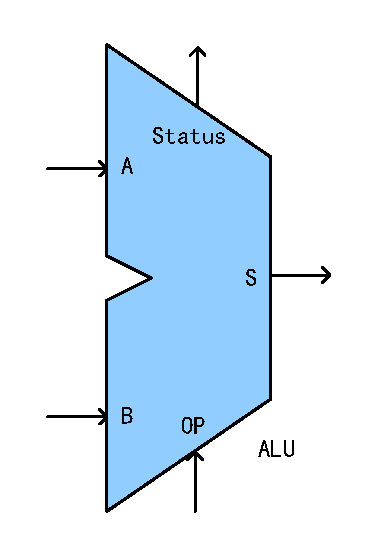
\includegraphics[width=0.3\textwidth]{picture/ALU.pdf}
    \caption{ALU Block Diagram}     
    \label{fig:ALU}
\end{figure}

Where \texttt{A} and \texttt{B} are 32 bits input buses, 
\texttt{S} is a 32 bits output bus, 
\texttt{OP} is a 2 bits command signal, 
and \texttt{Status} is a Output Signal represent NVCZ (we just consider N here, so it is 1 bit).

For the operation of ALU, we can see from Table \ref{tab: Operation Table}.

Thus, we set the inputs and outputs \texttt{ports} of the \texttt{entity} as follow:
\begin{lstlisting}[style=vhdl,columns=fullflexible]
entity ALU is
    port(
        op:in std_logic_vector(1 downto 0);
        a,b: in std_logic_vector(31 downto 0);
        s: out std_logic_vector(31 downto 0);
        n: out std_logic
    );
end entity;
\end{lstlisting}
    
Whenever instructed by the processor, the ALU performs an operation 
(we consider addition and subtraction, and the detailed table will be given below) on one or more values. These values, called operands , 
are typically obtained from two registers, or from one register and a memory location. 
The result of the operation is then placed back into a given destination register 
or memory location. The status outputs indicate any special attributes about the operation, 
such as whether the result was zero, negative, or if an overflow or carry occurred. \cite{catsoulis2005designing} 
\vspace{2cm}
\begin{table}[htbp]
    \centering
    \caption{Operation Table}
    \label{tab: Operation Table}
    \begin{tabular}{@{}ccc@{}}
    \toprule
    \textbf{OP} & \textbf{S} & \textbf{Remark} \\ \midrule
    00              & S=A+B      & ADD             \\
    01              & S=B        & B               \\
    10              & S=A-B      & SUB             \\
    11              & S=A        & A               \\ \bottomrule
    \end{tabular}
\end{table}

Therefore, we build the \texttt{architecture} of ALU in \texttt{\bf{ALU.vhd}}.

\begin{lstlisting}[style=vhdl,columns=fixed]
architecture behav of ALU is
    signal sign: std_logic_vector(31 downto 0);
begin 

    process (a,b,op)
      begin 
        case op is 
            when"00" => sign <=std_logic_vector(signed(a)+signed(b)); 
            when"01" => sign <= b; 
            when"10" => sign <=std_logic_vector(signed(a)-signed(b)); 
            when"11" => sign <= a;
            when others => sign <= a; 
        end case ;
    end process;

    N <= sign(31);
    s <= sign;

end architecture; 
\end{lstlisting}

%%%%%%%%%%%%%%%%%%%%%%%%%%%%%%%%%%%%%%%%%%%%%%%%%%%%%%%%%%%%%%%%%%%%%%%%%%
\subsection{Register File (Banc de Registres)}

\subsubsection{Design Register File}

Registers are temporary storage locations inside the CPU 
that hold data and addresses.

The register file is the component that 
contains all the general purpose registers 
of the microprocessor. A few CPUs also place 
special registers such as the PC and the status 
register in the register file. Other CPUs keep 
them separate.\cite{dumas2005computer}

A symbolic representation of an Register File is shown in Figure \ref{fig:RF}.


Where \texttt{Clk} is a clock Signal; \texttt{Rst} is a asynchrone reset signal which active at high level;
\texttt{WE} is a enable signal of writing datas and \texttt{Rw} is a 4 bits address bus of writing register;
\texttt{W}, \texttt{A} and \texttt{B} are 32 bits data buses; \texttt{Ra} and \texttt{Rb} are 4 bits address buses of reading register.

Thus, the \texttt{ports} of the \texttt{entity} we defined as follow:

\begin{lstlisting}[style=vhdl]
entity Register_File is 
	port (
		clk, rst, WE : in  std_logic ; 
		Ra, Rb, Rw : in std_logic_vector(3 downto 0);
		A, B : out std_logic_vector(31 downto 0);
		W : in std_logic_vector(31 downto 0)
	);
end entity;
\end{lstlisting}

\begin{figure}[h]
    \centering
    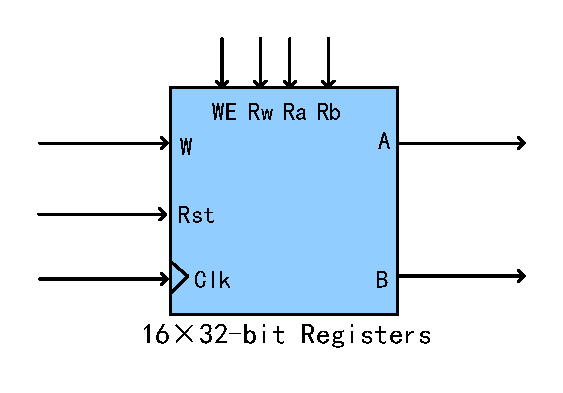
\includegraphics[width = 0.5\textwidth]{picture/16Register.pdf}
    \caption{Register File Block Diagram}     
    \label{fig:RF}
\end{figure}

When \texttt{WE}$ = 1$, which means \textit{enabel to write}, so that we need to write data from bus \texttt{W} to the register on the address \texttt{Rw};
And when \texttt{WE}$= 0$, we will do nothing.
As for reading, it will be done in a combinatorial and simultaneous way.

Therefore, we build the \texttt{architecture} of Register File in \textbf{Registre\_File.vhd}.

\begin{lstlisting}[style=vhdl]
architecture behav of Register_File is
	type matrix is array(15 downto 0) of std_logic_vector(31 downto 0);
	function init_banc return matrix is
		variable result : matrix;
	begin
		for i in 14 downto 0 loop
			result(i) := (others=>'0');
		end loop;
			result(15):=X"00000030";
		return result;
	end init_banc;

	signal Banc: matrix:=init_banc;
begin
	
	A <= Banc(to_integer(unsigned(Ra))); 
	B <= Banc(to_integer(unsigned(Rb))); 

	process(clk, rst) 
	begin 
        if rst ='1' then 
            for i in 14 downto 0 loop
                Banc(i) <= (others=>'0');
            end loop;
                Banc(15)<=X"00000030";
            
        elsif rising_edge(clk) then 
            if WE = '1' then 
                Banc(to_integer(unsigned(Rw)))<=W; 
            end if; 
        end if; 
	end process; 

end architecture;
\end{lstlisting}

\subsubsection{Assemble ALU and Register File}
\label{sec:Assemble ALU and Register File}

We will assemble these two component we have already finished as Figure \ref{fig:AsmbALURF}.

\begin{figure}[htp]
    \centering
    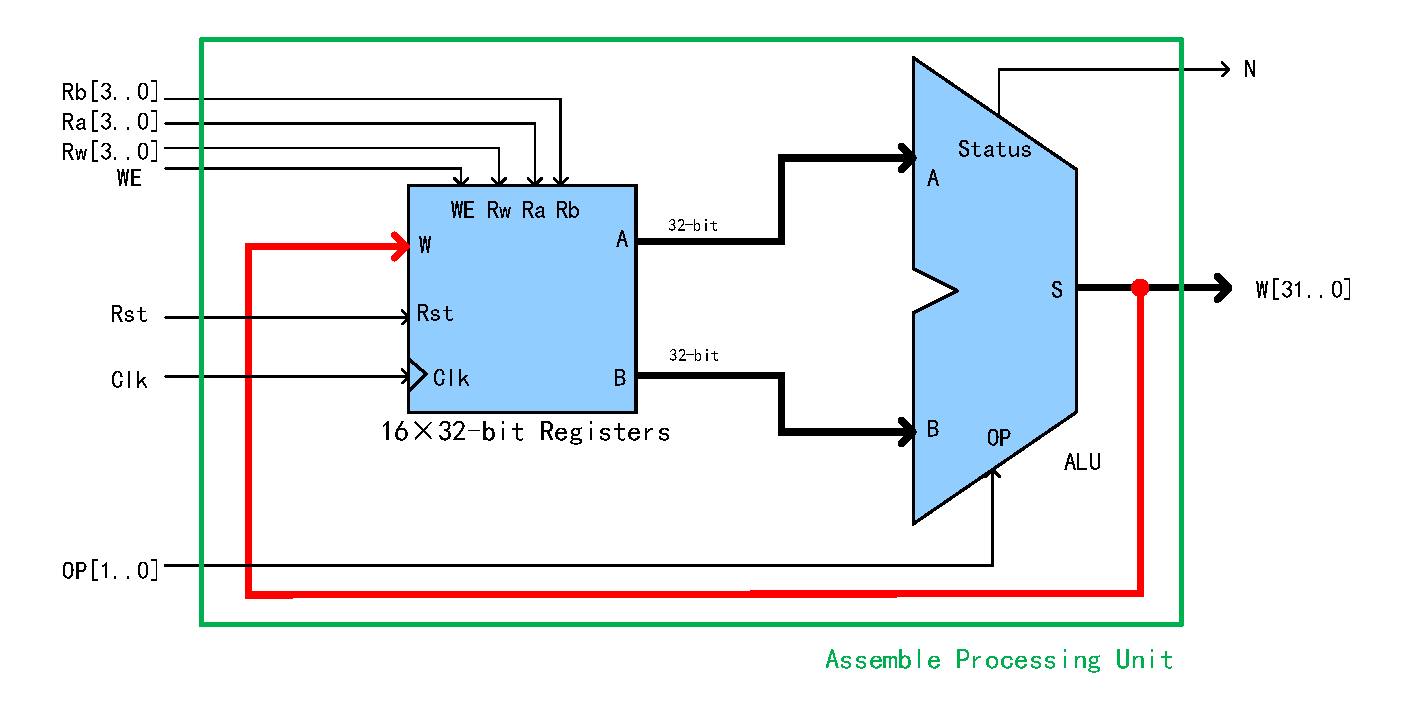
\includegraphics[width = 0.8\textwidth]{picture/AsmbALURF.pdf}
    \caption{Assemble ALU and Register File Block Diagram}     
    \label{fig:AsmbALURF}
\end{figure}

The \texttt{entity} and \texttt{architecture} of \textbf{Assemble\_ALU\_and\_Register\_File.vhd} shows below.

\begin{lstlisting}[style=vhdl, breaklines]
entity Assemble_ALU_and_Register_File is 
    port (
        clk, rst, WE : in  std_logic ; 
        Ra, Rb, Rw : in std_logic_vector(3 downto 0);
        W : out std_logic_vector(31 downto 0);
        N : out std_logic; 
        op : in std_logic_vector(1 downto 0)
    );
end entity;
  
architecture behave of Assemble_ALU_and_Register_File is
    signal busA,busB, busW : std_logic_vector(31 downto 0);
begin
  
    Register_File : entity work.Register_File port map(clk=>clk, rst=>rst, WE=>We, Ra=>Ra, Rb=>Rb, Rw=>Rw, A=>busA, B=>busB, W=>busW); 

    ALU : entity work.ALU port map(a => busA, b=> busB, s => busW, op => op, n => n); 

    W <= busw; 
  
end architecture;
\end{lstlisting}

 And based on the textbench \textbf{Assemble\_ALU\_and\_Register\_File\_tb.vhd} and command file \textbf{Assemble\_ALU\_and\_Register\_File\_test.do}, we test some operations: 
\begin{center}
    \texttt{R(1) = R(15)} \\
    \texttt{R(1) = R(1) + R(15)}\\
    \texttt{R(2) = R(1) + R(15)}\\
    \texttt{R(3) = R(1) – R(15)}\\
    \texttt{R(5) = R(7) – R(15)} 
\end{center}

The simulation result is shown in Figure \ref{fig:AsmbALURFres}. Detailed waves can be found 
as Figure \ref{fig:ModelSim_ assemble_processing_unit_tb(test_bench)} in Appendices \ref{AppendicesA}.

\begin{figure}[htp]
    \centering
    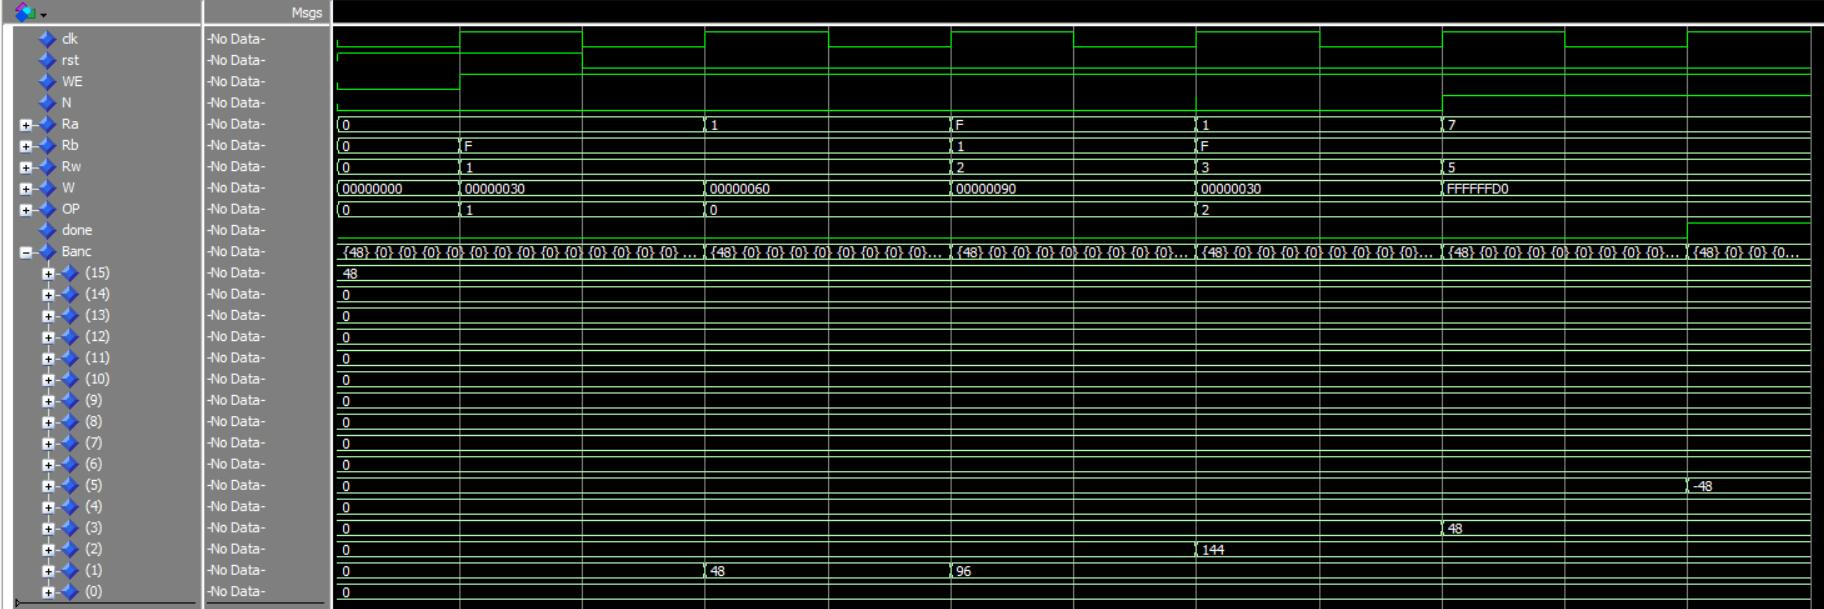
\includegraphics[width=1\textwidth]{picture/AsmbALURFres.jpg}
    \caption{Simulation Waves of Assemble ALU and Regist\_File}     
    \label{fig:AsmbALURFres}
\end{figure}

%%%%%%%%%%%%%%%%%%%%%%%%%%%%%%%%%%%%%%%%%%%%%%%%%%%%%%%%%%

\subsection{2 to 1 Multiplexer (Multiplexeur 2 vers 1)}

This multiplexer has a generic parameter \texttt{N} fixing 
the size of the data input and output. A symbolic representation 
of the multiplexer is shown in Figure \ref{fig:mux21}.

\begin{figure}[htp]
    \centering
    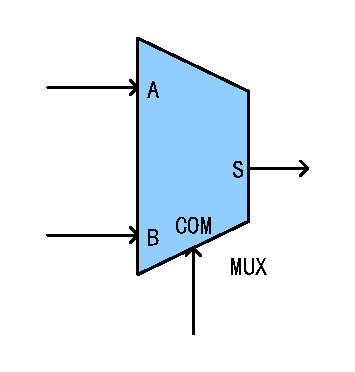
\includegraphics[width=0.3\textwidth]{picture/mux21.pdf}
    \caption{2 to 1 Multiplexer}     
    \label{fig:mux21}
\end{figure}

Where \texttt{A} and \texttt{B} are data inputs, \texttt{S} is data output, and they are all \texttt{N-bit};
\texttt{COM} is a choose signal which is 1 bit. The choose table is as below.

\begin{table}[h]
    \centering
    \caption{MUX Choose Table}
    \label{tab: Choose Table}
    \begin{tabular}{@{}cc@{}}
    \toprule
    \textbf{COM} & \textbf{S} \\ \midrule
    0            & S=A        \\
    1            & S=B        \\ \bottomrule
    \end{tabular}
\end{table}

So we build the component \texttt{MUX} in \textbf{MUX.vhd}.

\vspace{3mm}
\begin{lstlisting}[style=vhdl]
entity MUX is 
    generic (N : positive :=32);

    port (
        S : out std_logic_vector(N-1 downto 0);
        A, B : in std_logic_vector(N-1 downto 0);
        COM : in std_logic
    );
end entity MUX;
  
architecture behave of MUX is
begin
  
    process(A,B,COM)
    begin 
        if COM = '0' then S <= A; 
        elsif COM='1' then S <= B; 
        end if; 
    end process; 
  
end architecture;
\end{lstlisting}

%%%%%%%%%%%%%%%%%%%%%%%%%%%%%%%%%%%%%%%%%%%%%%%%

\subsection{Sign Extension (Extension de Signe)}

This module is used to extend the sign of an input coded 
on \texttt{N bits} to \texttt{32 bits}. It therefore has a generic parameter 
fixing the value of \texttt{N}. A symbolic representation 
of the multiplexer is shown in Figure \ref{fig:SignExtension}.

\begin{figure}[htp]
    \centering
    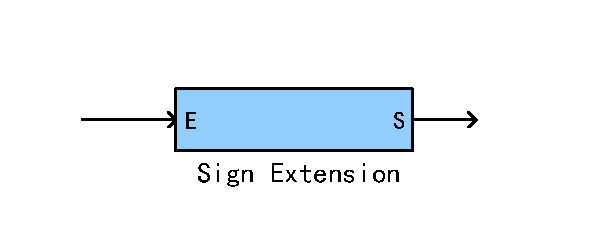
\includegraphics[width=0.5\textwidth]{picture/SignExtension.pdf}
    \caption{Sign Extension Block Diagram}     
    \label{fig:SignExtension}
\end{figure}

Where \texttt{E} is a \texttt{N-bit} data input bus and \texttt{S} is a 32-bit output bus.

And part of its code in \textbf{Sign\_Extension.vhd} shows below.

\begin{lstlisting}[style=vhdl]
entity Sign_Extension is 
    generic (N : positive :=8);
    port (			
        S : out std_logic_vector(31 downto 0);
        E : in std_logic_vector(N-1 downto 0)			
    );
end entity;
  
architecture behav of Sign_Extension is
begin
  
    process(E)
    begin 
        S(N-1 downto 0) <= E; 
        S(31 downto N) <= (others => E(N-1)); 
    end process; 
  
end architecture;
\end{lstlisting}

%%%%%%%%%%%%%%%%%%%%%%%%%%%%%%%%%%%%%%%%%%%%%%%%%%%%%%%%%%

\subsection{Data Memory (Mémoire de Données)}

This memory is used to load and store 64 32-bit words. A symbolic representation 
of the Memory is shown in Figure \ref{fig:DataMem}.

\begin{figure}[htp]
    \centering
    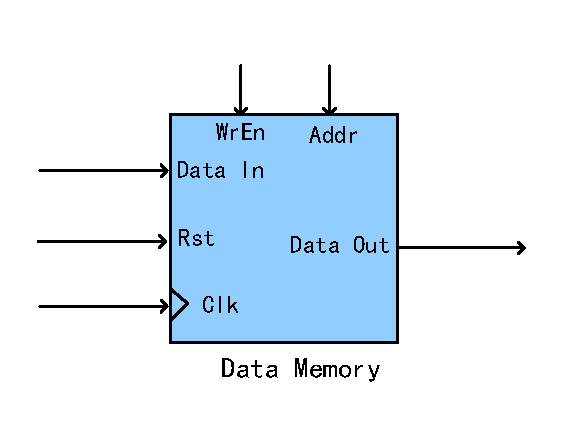
\includegraphics[width=0.5\textwidth]{picture/DataMem.pdf}
    \caption{Data Memory Block Diagram}     
    \label{fig:DataMem}
\end{figure}

Where \texttt{Clk} is a clock Signal; \texttt{Rst} is a asynchrone reset signal which active at high level;
\texttt{WrEn} is a enable signal of writing datas and \texttt{Addr} is a 6 bits address bus;
\texttt{Data In} and \texttt{Data Out} are 32 bits data buses;

Thus, the ports of the entity we defined as follow:

\begin{lstlisting}[style=vhdl]
entity Data_Memory  is 
	port (
		clk, rst, WE : in  std_logic ; 
		Addr : in std_logic_vector(5 downto 0);
		DataOut : out std_logic_vector(31 downto 0);
		DataIn : in std_logic_vector(31 downto 0)
	);
end entity;
\end{lstlisting}

Similar to Register File, when \texttt{WrEn}$=1$, it will write data from \texttt{Data In} to the \texttt{Addr} register;
and when \texttt{WrEn}$=0$, it will do nothing. As for reading, it will be done
in a combinatorial and simultaneous way.

Therefore, we build the \texttt{architecture} of Data Memory in \textbf{Data\_Memory.vhd}

\begin{lstlisting}[style=vhdl]
architecture behave of Data_Memory  is
	type matrix is array(63 downto 0) of std_logic_vector(31 downto 0);
	signal datas: matrix;
begin

	DataOut <= datas(to_integer(unsigned(Addr))); 
	process(clk, rst) 
	begin 
		if rst ='1' then 
			for i in 63 downto 0 loop
				datas(i) <= std_logic_vector(to_unsigned(i,32));
			end loop;
		elsif rising_edge(clk) then 
			if WE = '1' then 
				datas(to_integer(unsigned(Addr)))<=DataIn; 
			end if; 
		end if; 
	end process; 

end architecture;
\end{lstlisting}

%%%%%%%%%%%%%%%%%%%%%%%%%%%%%%%%%%%%%%%%%%%%%%%%%%

\subsection{Assemble Processing Unit (Assemblage Unité de Traitement)}

We assemble all the components we have finished before to make a Processing Unit.
All the signals are readable from the bolck diagram shown as Figure \ref{fig:AsmbUT}.
And we give the part of source code of \textbf{Assemble\_Processing\_Unit.vhd}.

\begin{figure}[htp]
    \centering
    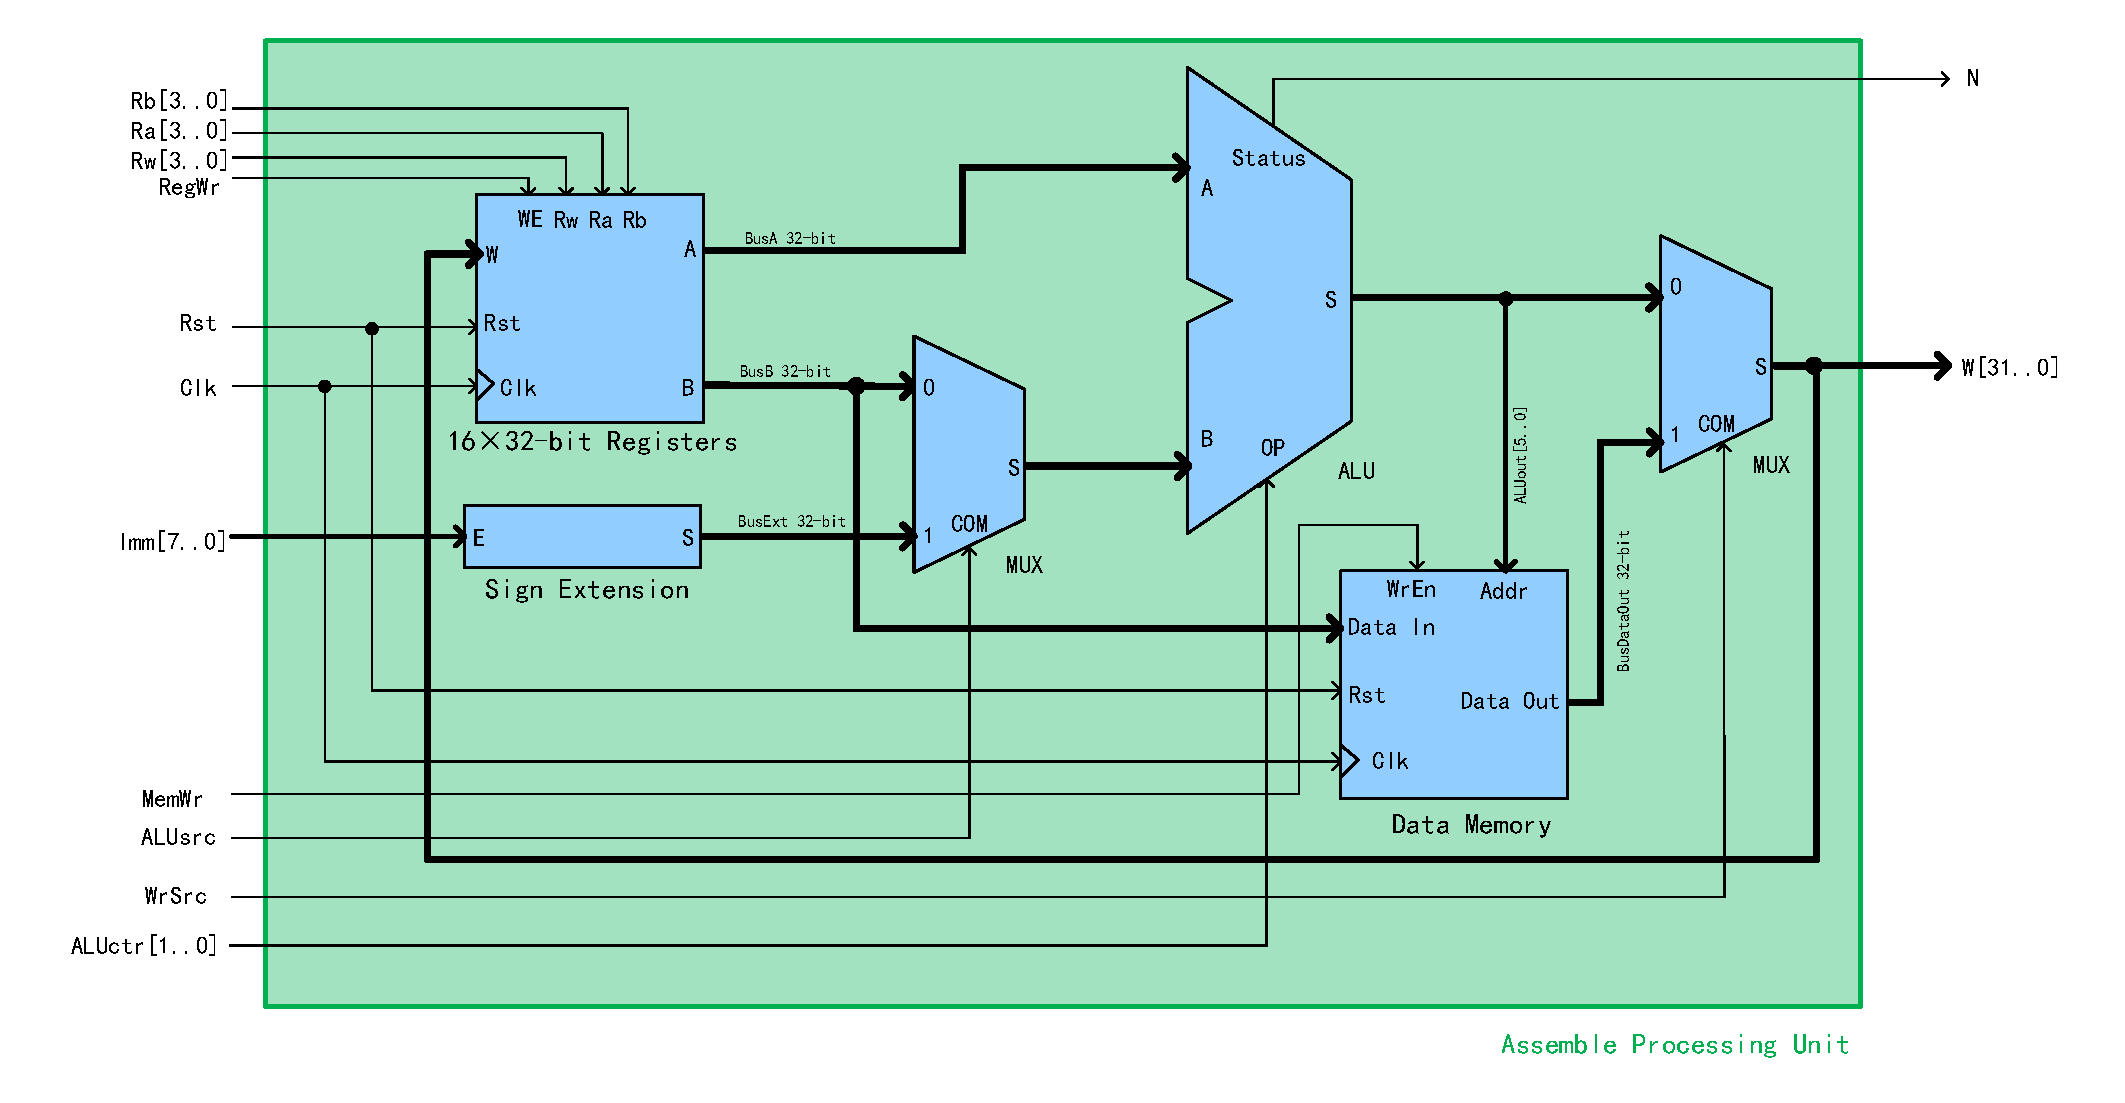
\includegraphics[width=1\textwidth]{picture/AsmbUT.pdf}
    \caption{Assemble Processing Unit Block Diagram}     
    \label{fig:AsmbUT}
\end{figure}

\begin{lstlisting}[style=vhdl, breaklines]
architecture behave of Assemble_Processing_Unit is
    signal busA,busB,ALUS,busExtension,busMux, busW : std_logic_vector(31 downto 0);
    signal DataOut: std_logic_vector(31 downto 0);
begin
  
    Register_File : entity work.Register_File port map(Clk => clk, rst => rst, WE=> RegWr, Ra => Ra, Rb => Rb, Rw => Rw, A => busA, B => busB, W=> busW); 
  
    ALU : entity work.ALU port map(A => busA, B=> busMux, S => ALUS, OP => ALUctr, N => N); 
  
    Sign_Extension : entity work.Sign_Extension port map (E => Imm, S => busExtension);
  
    MUX1 : entity work.MUX port map (A => busB, B=> busExtension, S=> busMux, COM => ALUSrc); 
  
    MUX2 : entity work.MUX port map (A => ALUS, B=> DataOut, S=> busW, COM => WrSrc);
  
    Data_Memory : entity work.Data_Memory port map (Clk => clk, rst => rst, Addr => ALUS(5 downto 0), WE => MemWr, DataIn => busB, DataOut => DataOut); 
    
    W <= busw; 
  
end architecture;
\end{lstlisting}

\clearpage
\section{Instruction Management Unit (Unité de gestion des instructions)}

\subsection{Design Instruction Management Unit}

The 32-bit instruction management unit possesses some properties:
\begin{itemize}
    \item An instruction memory of 64 words of 32 bits similar to that 
    of the processing unit.
    \item There is no write data bus and Write Enable.
    \item A 32-bit register (PC register) which has a clock and a
    asynchronous reset (active at high level).
    \item An extension unit of 24 to 32 signed bits similar to the component \texttt{Extension} described
    previously.
\end{itemize}

A symbolic representation of an Instruction Management Unit
is shown in Figure \ref{fig:IMU}.

\begin{figure}[htp]
    \centering
    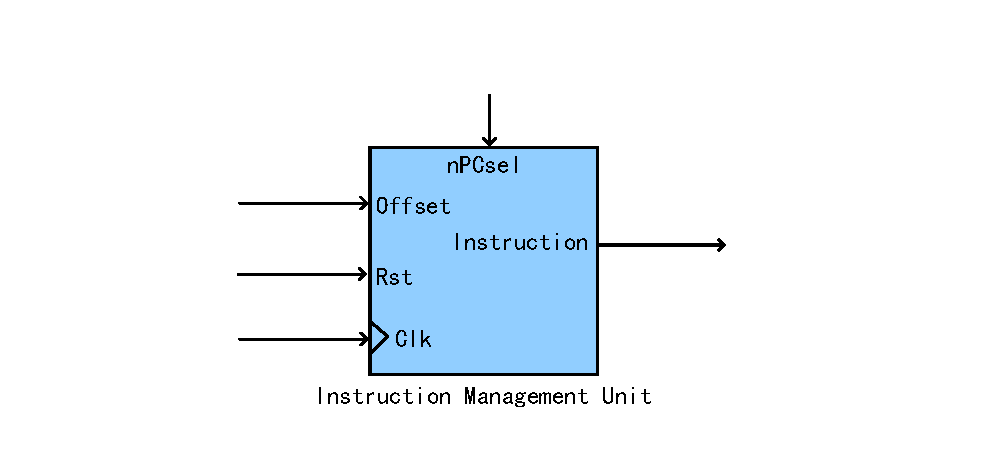
\includegraphics[width=0.5\textwidth]{picture/IMU.pdf}
    \caption{Instruction Management Unit Block Diagram}     
    \label{fig:IMU}
\end{figure}

Abstracted by the given block diagram, 
the function of the instruction management unit can be 
discribed as follow:
\begin{equation*}
    \texttt{PC} = \begin{cases}
        \texttt{PC} + 1 & \texttt{nPCsel} = 0 \\
        \texttt{PC} + 1 + \texttt{offset} & \texttt{nPCsel} = 1
    \end{cases}
\end{equation*} 

Because the instructions given are 24-bit, we need to use component \texttt{Extension} to extend them to 32-bit.
After that, we store these 32-bit instructions in memory by \texttt{Datamemory}.

The part of the source in \textbf{Instruction\_Management\_Unit.vhd} will be given below.
\begin{lstlisting}[style=vhdl,breaklines]
architecture behave of Instruction_Management_Unit is
	signal PC, S : std_logic_vector(31 downto 0);  
begin

	Instruction_memory : entity work.instruction_memory port map (PC=> PC, Instruction=> Instruction); 
	Sign_Extension  : entity work.Sign_Extension  generic map(N=> 24) port map ( E => Offset, S => S); 

	process(clk, rst) 
	begin 
        if rst ='1' then 
            PC <= (others => '0'); 
        elsif rising_edge(clk) then 
            if nPCsel = '0' then 
                PC <= std_logic_vector(unsigned(PC)+1);	
            else 
                PC <= std_logic_vector(unsigned(PC)+1+ unsigned(S));	
            end if; 
        end if; 
	end process; 
end architecture;
\end{lstlisting}

And here is the code \textbf{instruction\_memory.vhd} in Appendices \ref{AppendicesA}.

\begin{lstlisting}[style=vhdl, columns=fixed,breaklines]
library IEEE;
use IEEE.std_logic_1164.all;
use IEEE.numeric_std.all;

entity instruction_memory is
    port(
        PC: in std_logic_vector(31 downto 0);
        Instruction: out std_logic_vector(31 downto 0)
    );
end entity;

architecture RTL of instruction_memory is
    type RAM64x32 is array(0 to 63) of std_logic_vector(31 downto 0);
    
function init_mem return RAM64x32 is 
    variable result : RAM64x32;
begin
    for i in 63 downto 0 loop
        result(i) := (others => '0');
    end loop;					 -- PC        -- INSTRUCTION  
        result(0) := x"E3A01020";-- 0x0 _main -- MOV R1,#0x20 
        result(1) := x"E3A02000";-- 0x1		  -- MOV R2,#0x00 
        result(2) := x"E6110000";-- 0x2 _loop -- LDR R0,0(R1)  
        result(3) := x"E0822000";-- 0x3		  -- ADD R2,R2,R0 
        result(4) := x"E2811001";-- 0x4		  -- ADD R1,R1,#1 
        result(5) := x"E351002A";-- 0x5		  -- CMP R1,0x2A  
        result(6) := x"BAFFFFFB";-- 0x6		  -- BLT loop 	 
        result(7) := x"E6012000";-- 0x7		  -- STR R2,0(R1) 
        result(8) := x"EAFFFFF7";-- 0x8		  -- BAL main	 
    return result;
end init_mem;	

signal mem: RAM64x32 := init_mem;

begin 
    Instruction <= mem(to_integer(unsigned(PC)));
end architecture;
	
\end{lstlisting}

\subsection{Simulation for Instruction Management Unit}
\label{sec:Simulation for Instruction Management Unit}

We build the testbench in order to test whether this unit work properly.


We mainly test the instruction such as
\begin{center}
        \texttt{PC} <= \texttt{PC} + 1 \\
        \texttt{PC} <=\texttt{PC} + 1 + \texttt{offset}
\end{center}
and change the value of \texttt{offset}$=\{1,-1\}$.

Given the code of the testbench \textbf{Instruction\_Management\_Unit\_tb.vhd} as follow.
\begin{lstlisting}[style=vhdl,columns=fixed, breaklines]
library ieee;
use ieee.std_logic_1164.all;
use ieee.numeric_std.all;

entity Instruction_Management_Unit_tb IS  
end entity ;
    
architecture BENCH of Instruction_Management_Unit_tb is
    signal Instruction : std_logic_vector(31 downto 0);
    signal Clk         : std_logic := '0';
    signal rst, nPCsel : std_logic;
    signal Offset      : std_logic_vector(23 downto 0);
    signal Done        : boolean := False; 
    constant Period    : time := 20 ns;
begin
    
    UUT : entity work.Instruction_Management_Unit port map(clk=>clk, rst=> rst, nPCsel =>nPCsel, Offset => Offset,Instruction => Instruction); 
    
    CLK <= '0' when Done else not CLK after Period / 2;
    Rst <= '1', '0' after 5 ns; 
    
    process
    begin
        
        nPCsel<= '0'; 
        Offset <= (others => '0'); -- PC <= PC + 1 
        wait for 20 ns;
        
        nPCsel<= '0'; 
        Offset <= (others => '0'); -- PC <= PC + 1 
        wait for 20 ns;
        
        nPCsel<= '1'; 
        Offset <= x"000001"; -- PC <= PC + 1 + Offset 1 
        wait for 20 ns;
        
        nPCsel<= '0'; 
        Offset <= (others => '0'); -- PC <= PC + 1
        wait for 20 ns;
        
        nPCsel<= '1'; 
        Offset <= x"FFFFFF"; -- PC <= PC + 1 + Offset -1 
        wait for 20 ns;
        
        nPCsel<= '0'; 
        Offset <= (others => '0'); -- PC <= PC + 1 
        wait for 20 ns;
        
        Done <= True; 
        wait;
        
    end process;
    
end architecture;    
\end{lstlisting}

With the command file \textbf{Instruction\_Management\_Unit\_test.do}, the waves of the simulation are shown as Figure \ref{fig:IMUres}. Detailed waves can be found as Figure \ref{fig:ModelSim_ insmanagement_tb(bench)} in Appendices \ref{AppendicesA}.

\begin{figure}[htp]
    \centering
    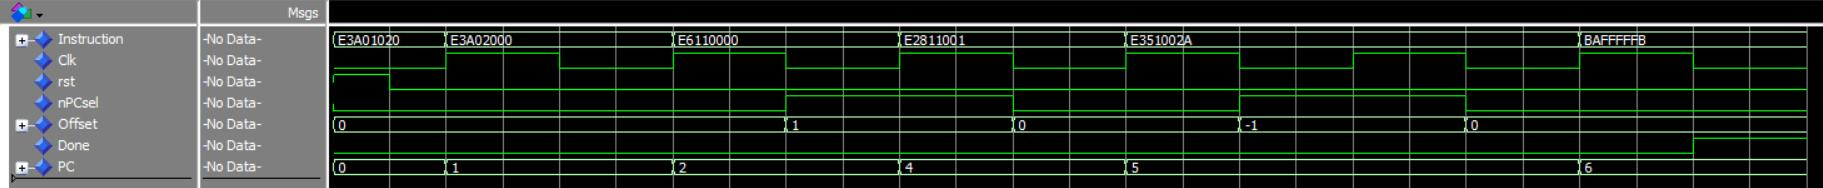
\includegraphics[width=1\textwidth]{picture/IMUres.jpg}
    \caption{Simulation of Instruction Management Unit}     
    \label{fig:IMUres}
\end{figure}

It can be seen clearly that \texttt{PC} change itself as we expected.


\clearpage
\section{Control Unit (Unité de Contrôle)}

The control unit consists of a 32-bit register and a combinatorial decoder.

\subsection{32-bit Register with Load Instruction (Registre 32-bit avec Commande de Chargement)}

This register will be used to store the state of the processor 
(Processor State Register, PSR).
In this project, we only consider the state which will be 
limited to the value of the \texttt{N flag} of the \textbf{ALU}.
A symbolic representation of this 32-bit register
is shown in Figure \ref{fig:32Register}.

\begin{figure}[htp]
    \centering
    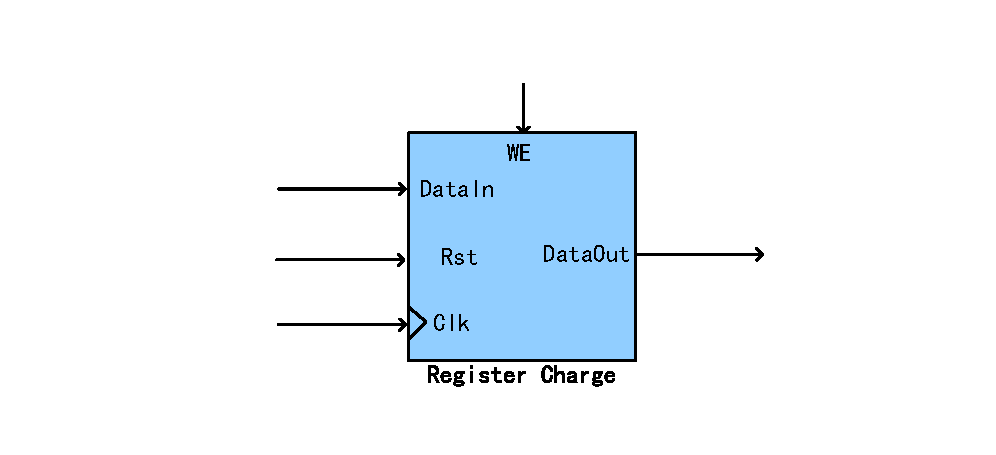
\includegraphics[width=0.4\textwidth]{picture/32Register.pdf}
    \caption{32-bit Register Block Diagram}     
    \label{fig:32Register}
\end{figure}

Where \texttt{DataIn} and \texttt{DataOut} are the 32-bit buses for 
instruction input and outpout respectively, \texttt{WE} is enable signal
for charge command.

Based on the analysis above, we can draw the equation:
\begin{equation*}
    \texttt{DataOut} = \begin{cases}
        \texttt{DataOut} & \texttt{WE} = 0 \\
        \texttt{DataIn} & \texttt{WE} = 1
    \end{cases}
\end{equation*} 

It's not hard to synthesize the code. We show the part of the code of this component in \textbf{Registre\_Charge.vhd}.

\begin{lstlisting}[style=vhdl]
architecture behave of Register_Charge is
begin
    
    process(clk, rst) 
    begin 
        if rst ='1' then 
            DataOut <= (others => '0'); 
        elsif rising_edge(clk) then 
            if WE = '1' then 
                DataOut <= DataIn;	
            end if; 
        end if; 
    end process; 
    
end architecture;
\end{lstlisting}


\subsection{Instruction Decoder (Decodeur d’Instructions)}
\label{sec:Instruction Decoder}

This combinatorial module generates the control signals for 
the processing unit, the instruction management unit, 
as well as the PSR register(32-bit register), which all described
previously.

A symbolic representation of decoder
is shown in Figure \ref{fig:decoder}.

\begin{figure}[htp]
    \centering
    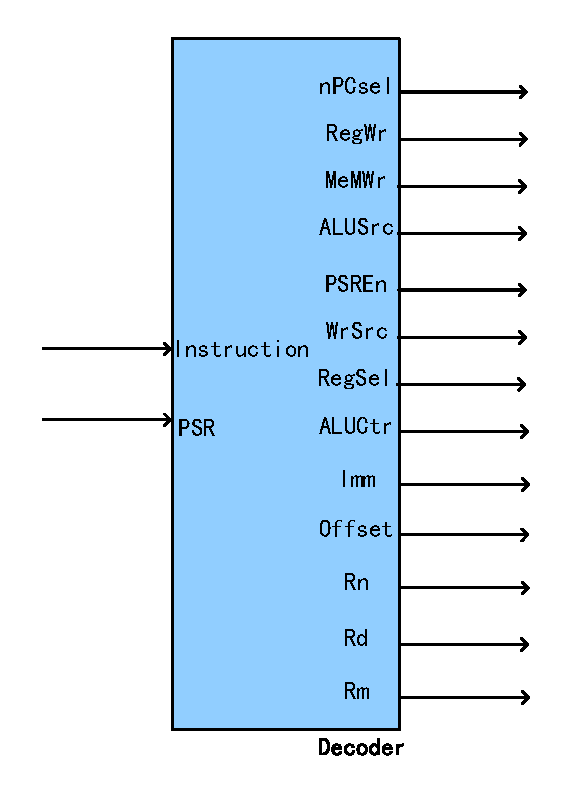
\includegraphics[width=0.4\textwidth]{picture/decoder.pdf}
    \caption{Decoder Block Diagram}     
    \label{fig:decoder}
\end{figure}

The values of these commands depend on the statement retrieved from 
the instruction memory, and possibly the state of the PSR register. 
The structure binary of the different instructions is described 
in the Appendix, and we completed it as Table \ref{tab:command}.

\begin{table}[htp]
    \caption{Commands}
    \label{tab:command}
    \resizebox{\textwidth}{!}
    {
        \begin{tabular}{@{}ccccccccc@{}}
        \toprule
        \textbf{INSTRUCTION} & \textbf{nPCSel} & \textbf{RegWr} & \textbf{ALUSrc} & \textbf{ALUCtr} & \textbf{PSREn} & \textbf{MemWr} & \textbf{WrSrc} & \textbf{RegSel} \\ \midrule
        ADDi                 &       0         &          1     &      1          &       00         &     0          &       0        &      0         &   0             \\
        ADDr                 &       0         &         1      &      0          &      00          &      0         &        0       &       0        &  0              \\
        BAL                  &         1       &        0       &     0           &    00            &     0          &     0          &     0          &    0            \\
        BLT                  &         0       &           0    &          0      &      00         &       0        &         0      &        0       &      0          \\
        CMP                  &       0         &    0           &    1            &    10           &     1          &     0          &        0       &   0             \\
        LDR                  &         0       &      1         &         1       &      00          &        0       &         0      &       1        &    0            \\
        MOV                  &         0       &       1        &           1     &         10       &       0        &     0          &        0       &      0          \\
        STR                  &         0       &   0            &       1         &       00         &       0        &       1        &       0        &      1          \\ \bottomrule
        \end{tabular}
    }
\end{table}

The ARM instruction set formats are shown in the Appendices \ref{AppendicesA}.

And we focus on the instructions such as
\begin{lstlisting}[style = Arm, columns = fixed]
    LDR Rd, [Rn, #Offset]   @ LDR (Immediate)
    STR Rd, [Rn, #Offset]   @ STD (Immediate)
    B       label           @ B (Always)
    BLT     label           @ B (If Less Than)
\end{lstlisting}

These instruction set formats are shown as Figure \ref{fig:AISFIP}, and more detailed information will be shown in the Appendices \ref{AppendicesA}.

\begin{figure}[htp]
    \centering
    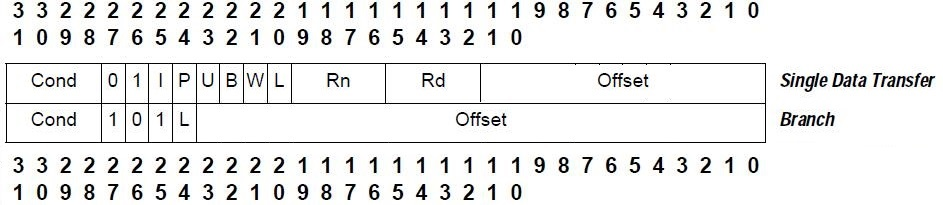
\includegraphics[width=1\textwidth]{picture/ARM instruction set formats in project.jpg}
    \caption{Load, Store and Branch Instruction Set Formats}     
    \label{fig:AISFIP}
\end{figure}

The single data transfer instructions are used to load or store single bytes or words of
data. The memory address used in the transfer is calculated by adding an offset to or
subtracting an offset from a base register.

The result of this calculation may be written back into the base register if auto-indexing
is required.

Branch instructions contain a signed 2’s complement 24 bit offset. This is shifted left
two bits, sign extended to 32 bits, and added to the PC. The instruction can therefore
specify a branch of +/- 32Mbytes. The branch offset must take account of the prefetch
operation, which causes the PC to be 2 words (8 bytes) ahead of the current instruction.
Branches beyond +/- 32Mbytes must use an offset or absolute destination which has
been previously loaded into a register. In this case the PC should be manually saved in
R14 if a Branch with Link type operation is required.

Thus, for these 4 instructions, bit assignments are as follow:\\
\begin{table}[h!]
    \centering
    \caption{LDR (Immediate) Bit Assignment}
    \label{tab:LDRBA}
    \begin{tabular}{|cccc|cccccccc|ccc|ccc|ccc|}
    \hline
    31 & 30 & 29 & 28 & 27 & 26                     & 25                     & 24                     & 23                     & 22                     & 21                     & 20 & 19     & ...    & 16    & 15     & ...    & 12    & 11      & ...      & 0      \\ \hline
    1  & 1  & 1  & 0  & 0  & \multicolumn{1}{c|}{1} & \multicolumn{1}{c|}{1} & \multicolumn{1}{c|}{0} & \multicolumn{1}{c|}{0} & \multicolumn{1}{c|}{0} & \multicolumn{1}{c|}{0} & 1  & \multicolumn{3}{c|}{Rn} & \multicolumn{3}{c|}{Rd} & \multicolumn{3}{c|}{Offset} \\ \hline
    \end{tabular}
\end{table}

\begin{table}[h!]
    \centering
    \caption{STR (Immediate) Bit Assignment}
    \label{tab:STRBA}
    \begin{tabular}{|cccc|cccccccc|ccc|ccc|ccc|}
    \hline
    31 & 30 & 29 & 28 & 27 & 26                     & 25                     & 24                     & 23                     & 22                     & 21                     & 20 & 19     & ...    & 16    & 15     & ...    & 12    & 11      & ...      & 0      \\ \hline
    1  & 1  & 1  & 0  & 0  & \multicolumn{1}{c|}{1} & \multicolumn{1}{c|}{1} & \multicolumn{1}{c|}{0} & \multicolumn{1}{c|}{0} & \multicolumn{1}{c|}{0} & \multicolumn{1}{c|}{0} & 0  & \multicolumn{3}{c|}{Rn} & \multicolumn{3}{c|}{Rd} & \multicolumn{3}{c|}{Offset} \\ \hline
    \end{tabular}
\end{table}

\begin{table}[h!]
    \centering
    \caption{B (Always) Bit Assignment}
    \label{tab:BALBA}
    \begin{tabular}{|cccc|cccc|ccllllllllllc|}
    \hline
    31 & 30 & 29 & 28 & 27 & 26 & 25                     & 24 & 23 & ...    &  ...   &   ...  & ... & ... & ... & ... & ... & ... & ... & ... & 0 \\ \hline
    1  & 1  & 1  & 0  & 1  & 0  & \multicolumn{1}{c|}{1} & 0  & \multicolumn{13}{c|}{Offset}                                             \\ \hline
    \end{tabular}
    
\end{table}

\begin{table}[h!]
    \centering
    \caption{B (If Less Than) Bit Assignment}
    \label{tab:BLTBA}
    \begin{tabular}{|cccc|cccc|ccllllllllllc|}
    \hline
    31 & 30 & 29 & 28 & 27 & 26 & 25                     & 24 & 23 & ...    &  ...   &   ...  & ... & ... & ... & ... & ... & ... & ... & ... & 0 \\ \hline
    1  & 0  & 1  & 1  & 1  & 0  & \multicolumn{1}{c|}{1} & 0  & \multicolumn{13}{c|}{Offset}                                             \\ \hline
    \end{tabular}
\end{table}

\vspace{3cm}
Based on the analysis above, we build the code of \textbf{Decoder.vhd}.
\begin{lstlisting}[style=vhdl,columns=fixed, breaklines]
entity Decoder  is
	port(
		Instruction, PSRout : in std_logic_vector(31 downto 0);
		Offset : out std_logic_vector(23 downto 0);
		Immediate : out std_logic_vector(7 downto 0);
		Rn, Rm, Rd : out std_logic_vector(3 downto 0);
		ALUctr : out std_logic_vector(1 downto 0);
		nPCsel, RegWr, ALUsrc, PSRen, MemWr, WrSrc, RegSel : out std_logic
	);
end entity;

architecture behave of Decoder  is
	type enum_instruction is (MOV, ADDi, ADDr, CMP, LDR, STR, BAL, BLT, XXX);
	signal instr_courante: enum_instruction;
begin

	Immediate <= Instruction(7  downto  0);
	Offset    <= Instruction(23 downto  0);
	Rn        <= Instruction(19 downto 16);
	Rd        <= Instruction(15 downto 12);
	Rm        <= Instruction(3  downto  0);
	process(Instruction)
	begin
		case Instruction(27 downto 26) is
			when "00"   => 
				case Instruction(25 downto 23) is
					when "001"          => instr_courante <= ADDr;
					when "101"          => 
						case Instruction(29) is
							when '1'    => instr_courante <= ADDi;
							when others => instr_courante <= XXX;
						end case;
					when "110" | "010"  => instr_courante <= CMP;
					when "111"          => instr_courante <= MOV;
					when others         => instr_courante <= XXX;
				end case;
									
			when "01"   => 
				case Instruction(20) is
					when '0'    => 
						case Instruction(29) is
							when '1'    => instr_courante <= STR;
							when others => instr_courante <= XXX;
						end case;
					when '1'    => instr_courante <= LDR;
					when others => instr_courante <= XXX;
				end case;
									
			when "10"   => 
				case Instruction(29 downto 28) is
					when "10"    => instr_courante <= BAL;
					when "11"    => instr_courante <= BLT;
					when others  => instr_courante <= XXX;
				end case;					   
			when others => instr_courante <= XXX;
		end case; 
	end process;
		
	process(instr_courante)
	begin
		-- MemWr et RegSel
		case instr_courante is
			when STR 	=> 	MemWr  <= '1';
						   	ALUSrc <= '1'; 
						   	RegSel <= '1';
			when others => 	MemWr  <= '0';
							RegSel <= '0';			
		end case;
		
		-- WrSrc
		case instr_courante is
			when LDR	=> 	WrSrc <= '1';
			when others => 	WrSrc <= '0';
		end case;
		
		-- PSRen et UALctr
		case instr_courante is
			when CMP 	=> 	PSRen  <= '1';
							ALUctr <= "10";
			when MOV	=> 	PSRen  <= '0';
							ALUctr <= "01";
			when others => 	PSRen  <= '0';
							ALUctr <= "00";
		end case;
		
		--UALsrc
		case instr_courante is
			when ADDr   => 	ALUsrc <= '0';
			when CMP    => 	ALUsrc <= Instruction(25);
			when others => 	ALUsrc <= '1';
		end case;
		
		-- RegWr
		case instr_courante is
			when ADDi | ADDr | LDR | MOV => RegWr <= '1';
			when others                  => RegWr <= '0';
		end case;
		
		-- nPCsel
		case instr_courante is
			when BAL    => nPCsel <= '1';
			when BLT    => nPCsel <= PSRout(31);
			when others => nPCsel <= '0';
		end case;
		
	end process;

end architecture;
\end{lstlisting}


At this point, all the components have been constructed. 
In the next part, we will try to assemble the processor by using these components.


\clearpage
\section{Assembly and Validation of Processor 
(Assemblage et Validation du Processeur)}

\subsection{Assemble Processor}
\label{sec:Assemble Processor}

We modifying the modeling of the processor by assembling its three main units
\begin{itemize}
    \item The instruction management unit
    \item The processing unit
    \item The control unit
\end{itemize}

Complete the previously designed processing unit by adding a
2-input 4-bit multiplexer controlled by the RegSel control signal
generated by the control unit. This multiplexer will be placed at the input of the address
Rb of the register file, as shown in the Figure \ref{fig:AsmbUTf}.

\begin{figure}[htp]
    \centering
    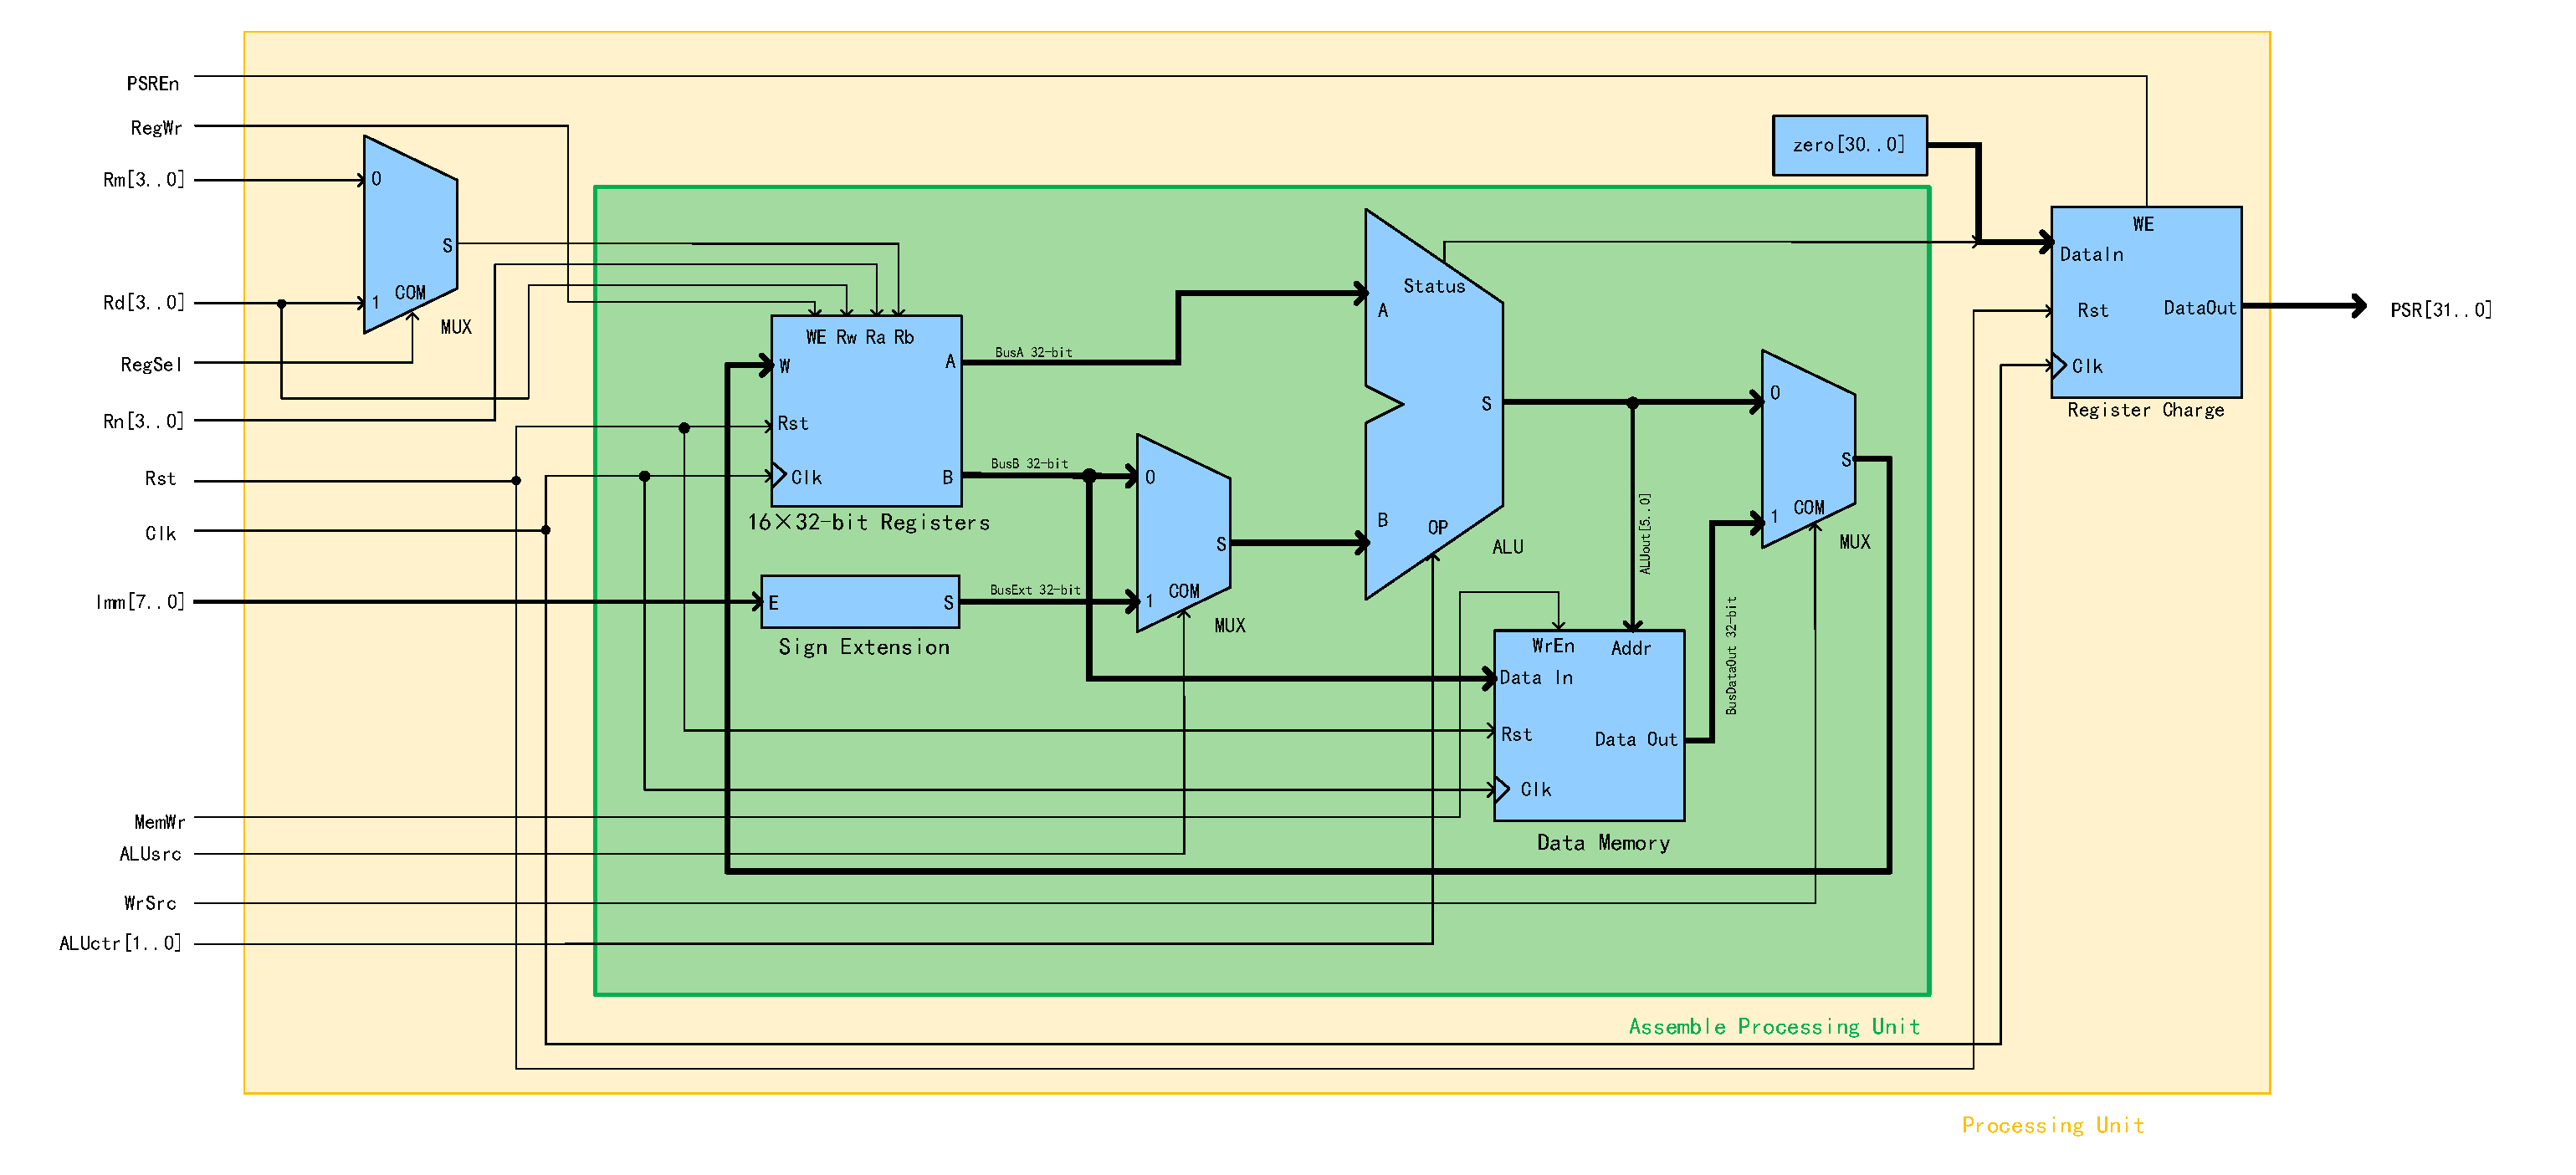
\includegraphics[width=1.5\textwidth, angle = 270]{picture/AsmbUTf.pdf}
    \caption{Processing Unit Block Diagram}     
    \label{fig:AsmbUTf}
\end{figure}

According to this block diagram, we modify the code for \textbf{Processing\_Unit.vhd}.

\begin{lstlisting}[style=vhdl, breaklines]
entity Processing_Unit is 
    port (
        clk, rst, MemWr, RegWr, ALUsrc, WrSrc ,RegSel, PSREn: in  std_logic ; 
        Rn, Rm, Rd : in std_logic_vector(3 downto 0);
        busout : out std_logic_vector(31 downto 0);--PSR[31..0]
        Imm : in std_logic_vector(7 downto 0); 
        ALUctr : in std_logic_vector(1 downto 0)
    );
end entity;
  
architecture behave of Processing_Unit is
    signal busA,busB,ALUS,busExtension,busMux, busW : std_logic_vector(31 downto 0);
    signal DataOut ,fl: std_logic_vector(31 downto 0);
    signal Rb : std_logic_vector(3 downto 0); 
    signal N: std_logic;
begin
  
    Register_File : entity work.Register_File port map(Clk => clk, rst => rst, WE=> RegWr, Ra => Rn, Rb => Rb, Rw => Rd, A => busA, B => busB, W=> busW); 
  
    ALU : entity work.ALU port map(A => busA, B=> busMux, S => ALUS, OP => ALUctr, N => N); 
  
    Sign_Extension : entity work.Sign_Extension port map ( E => Imm, S => busExtension);
  
    MUX1 : entity work.MUX port map (A => busB, B=> busExtension, S=> busMux, COM => ALUSrc); 
  
    MUX2 : entity work.MUX port map (A => ALUS, B=> DataOut, S=> busW, COM => WrSrc);
  
    Data_Memory : entity work.Data_Memory port map (Clk => clk, rst => rst, Addr => ALUS(5 downto 0), WE => MemWr, DataIn => busB, DataOut => DataOut); 
  
    MUX3 : entity work.MUX generic map( N=> 4) port map (A => Rm, B => Rd, COM => RegSel, S=> Rb); 
  
    Register_Charge : entity work.Register_Charge port map (clk => clk, rst => rst, WE => PSREn, DataIn => fl, DataOut => busout); 
  
    fl <= N&"000"&X"0000000";
  
end architecture;
\end{lstlisting}

With addition of \textbf{Processing\_Unit}, \textbf{Instruction\_Management\_Unit} and 
\textbf{Decoder}, the \textbf{Processor} can be assembled as Figure \ref{fig:PUs}. The detailed block diagram
will be given in the Appendices \ref{AppendicesA}.
\begin{figure}[htp]
    \centering
    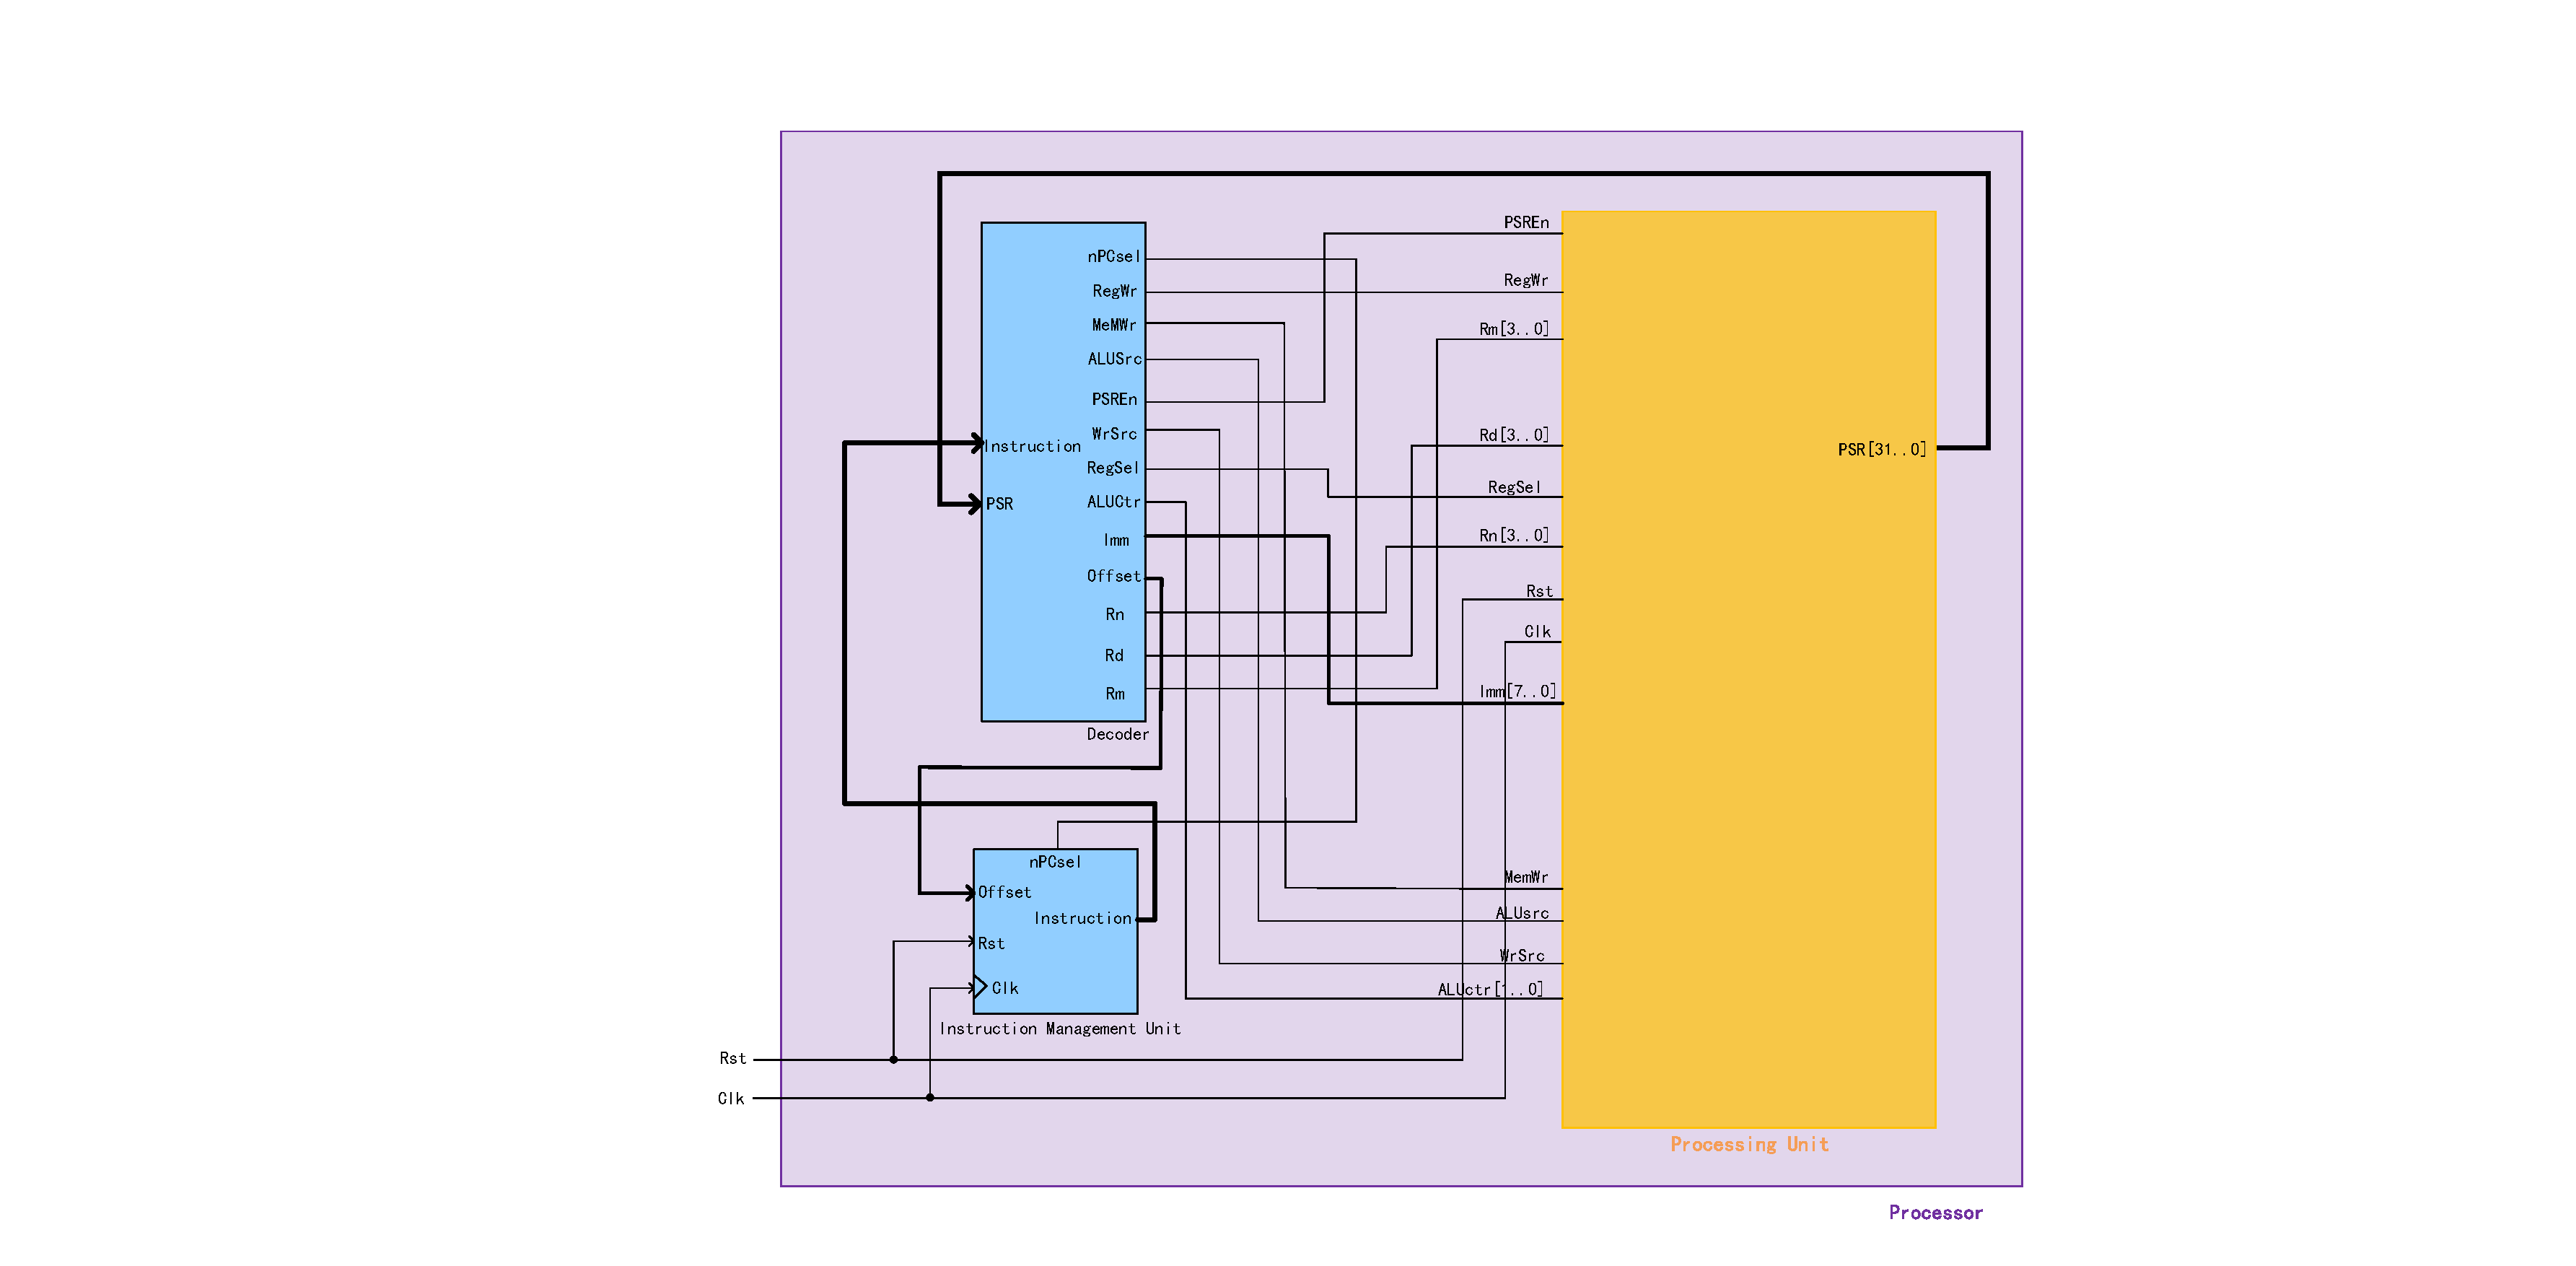
\includegraphics[width=1\textwidth]{picture/PUs.pdf}
    \caption{ProcessorBlock Diagram}     
    \label{fig:PUs}
\end{figure}

Thus, the core code for \textbf{Processor.vhd} is shown below.
\vspace*{1mm}
\begin{lstlisting}[style=vhdl,breaklines]
architecture behave of Processor is
    signal nPCSel, MemWr, RegWr, ALUsrc, WrSrc, RegSel, PSRen : std_logic ;
    signal ALUctr : std_logic_vector(1 downto 0);
    signal offset : std_logic_vector(23 downto 0);
    signal Immediate: std_logic_vector(7 downto 0);
    signal Instruction, busout : std_logic_vector(31 downto 0);--busout -> PSR
    signal Rn, Rd, Rm : std_logic_vector(3 downto 0); 
begin

    Processing_Unit : entity work.Processing_Unit port map(clk => clk, rst => rst, RegWr=> RegWr, Rn => Rn, Rd => Rd, Rm=> Rm, busout => busout, Imm => Immediate, ALUctr=> ALUctr, MemWr=> MemWr, ALUSrc=> ALUSrc,WrSrc=> WrSrc, RegSel=> RegSel, PSRen => PSRen); 

    Instruction_Management_Unit : entity work.Instruction_Management_Unit port map(Clk => clk, rst => rst, nPCSel=> nPCSel, Instruction=> Instruction, offset => offset); 

    Decoder  : entity work.Decoder  port map(RegWr=> RegWr, Rn => Rn, Rd => Rd, Rm=> Rm, psrout => busout, Immediate =>Immediate, ALUctr=> ALUctr, MemWr=> MemWr, ALUSrc=> ALUSrc, WrSrc=> WrSrc, RegSel=> RegSel, PSRen => PSRen, nPCSel=> nPCSel, Instruction=> Instruction, offset=> offset); 

end architecture;
\end{lstlisting}



\subsection{Simulate Processor}
\label{sec:Simulate Processor}

According to the testbench shown below, we run the simulation with command file \textbf{Processor\_test.do} and obtaine the waves as Figure \ref{fig:PUres}.
Detailed waves can be found as Figure \ref{fig:ModelSim_ processeur_tb(bench)} in Appendices \ref{AppendicesA}.
\begin{lstlisting}[style=vhdl]
library ieee;
use ieee.std_logic_1164.all;
use ieee.numeric_std.all;
    
entity Processor_tb is
end entity;
    
architecture test_bench of Processor_tb is
    signal clk, rst: std_logic;
    signal done : std_logic := '0';
    constant clk_period : time:= 10 ns;
begin
    
    UUT : entity work.Processor(behave)port map(clk => clk,rst => rst);

    rst <= '1', '0' after clk_period;
    
    clock : process is 
    begin
        if done = '0' then
            clk <= '0';
            wait for clk_period/2;
            clk <= '1';
            wait for clk_period/2;
        else
            wait;
        end if;
    end process;
    
    signal_gen : process is
    begin
        done <= '0';
        wait for clk_period*180;
        done <= '1';
        wait;
    end process;
        
end architecture;
\end{lstlisting}

\begin{figure}[htp]
    \centering
    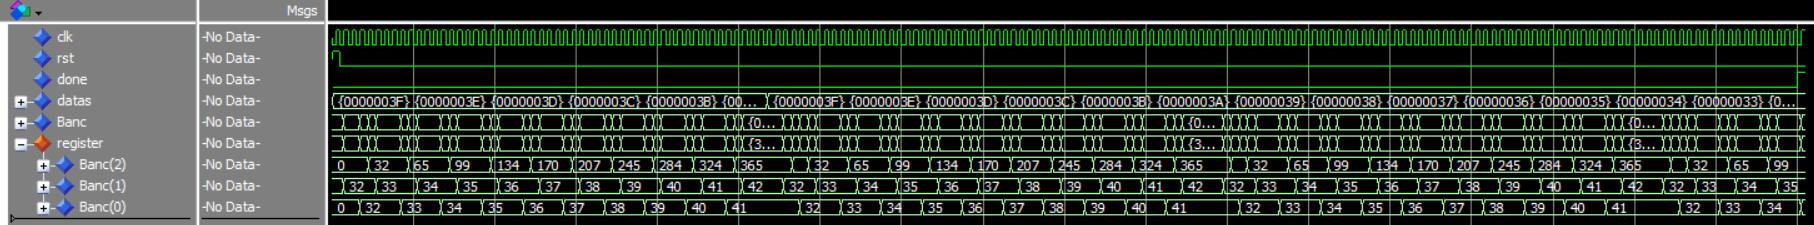
\includegraphics[width=1\textwidth]{picture/PUres.jpg}
    \caption{Simulation of Processing Unit}     
    \label{fig:PUres}
\end{figure}

\clearpage
\section{Test Processor Completely (Test Complet du Processeur)}
\label{sec:Test Processor Completely (Test Complet du Processeur)}
In this part, we will test the processor complement.

We first change the code Assembly given to the instruction code in \textbf{instruction\_memory2.vhd} according to Figure \ref{fig:AISF}.
\begin{lstlisting}[style = vhdl,columns=fixed]
result (0):=x"E3A00010";  -- 0x0 _main   -- MOV R0,#0x10
result (1):=x"E3A01001";  -- 0x1		 -- MOV R1,#0x01
result (2):=x"E6103000";  -- 0x2 _for    -- LDR R3,[R0]
result (3):=x"E6104001";  -- 0x3		 -- LDR R4,[R0,#1]
result (4):=x"E6004000";  -- 0x4		 -- STR R4,[R0]
result (5):=x"E6003001";  -- 0x5		 -- STR R3,[R0,#1]
result (6):=x"E2811001";  -- 0x6		 -- ADD R1,R1,#1
result (7):=x"E2800001";  -- 0x7		 -- ADD R0,R0,#1
result (8):=x"E351000A";  -- 0x8		 -- CMP R1,0xA
result (9):=x"BAFFFFF8";  -- 0x9		 -- BLT loop
result (10):=x"EAFFFFFF"; -- 0xA _wait	 -- BAL wait
\end{lstlisting}

After runing the simulation with command file \textbf{Processor\_test.do}, we obtaine waves as Figure \ref{fig:PUCres}.
Detailed waves can be found as Figure \ref{fig:ModelSim_ processeur_tb(bench) C} in Appendices \ref{AppendicesA}.

\begin{figure}[htp]
    \centering
    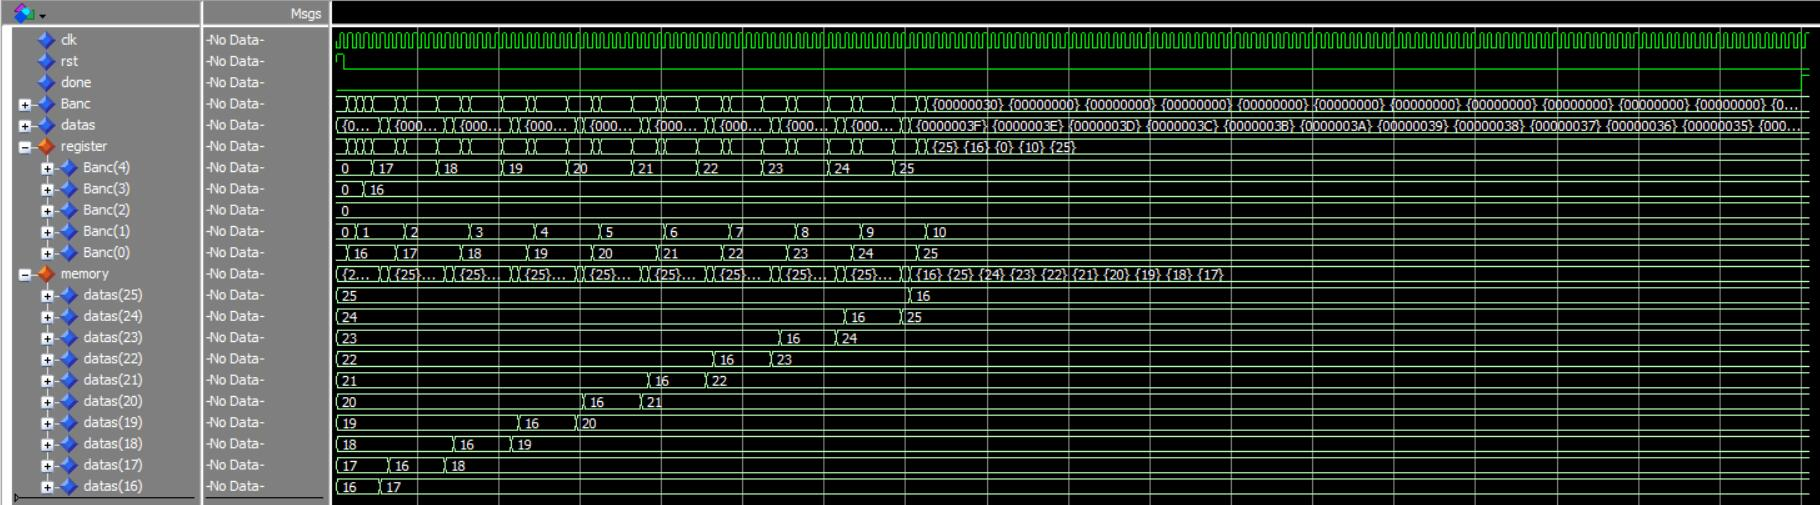
\includegraphics[width=1\textwidth]{picture/PUCres.jpg}
    \caption{Simulation Waves of Processing Unit Completely}     
    \label{fig:PUCres}
\end{figure}

\clearpage
\section{Increasing the Instruction Set (Augmentation du Jeu d'Instruction)}
\label{sec:Increasing the Instruction Set (Augmentation du Jeu d'Instruction)}

In this section, we have added additional command suffix support, including \texttt{EQ, NE, LT, GT}.
The detailed information is given in Table \ref{tab:Condition Code}.

\begin{table}[htbp]
    \centering
    \caption{Condtion Code}
    \label{tab:Condition Code}
    \begin{tabular}{@{}cccc@{}}
    \toprule
    \textbf{Code} & \textbf{Suffix} & \textbf{Flag} & \textbf{Meaning} \\ \midrule
    0000          & EQ              & Z=1           & equal            \\
    0001          & NE              & Z=0           & not equal        \\
    1011          & LT              & N=1           & less than        \\
    1100          & GT              & N=0           & greater than     \\ \bottomrule
    \end{tabular}
\end{table}

In order to match these changes, we need to modify the codes we have done before such as \textbf{ALU.vhd}, \textbf{Decoder.vhd} and \textbf{Data\_memory.vhd}
and rewrite the instructions in \textbf{instruction\_memory3.vhd}.

For \textbf{ALU.vhd}, we add an additional output port \texttt{Z} which indicated ZERO in Status.

For \textbf{Decoder.vhd}, we add the branch of \texttt{case} to make it decoder \texttt{EQ, NE, LT, GT} successfully
according to Table \ref{tab:Condition Code}.

For \textbf{Data\_memory.vhd}, we add the initialization for datas in memory as Table \ref{tab:datas in mem}.
\begin{table}[htbp]
    \centering
    \caption{Datas in Memory}
    \label{tab:datas in mem}
    \begin{tabular}{@{}cc@{}}
    \toprule
    \textbf{Address} & \textbf{Data} \\ \midrule
    0x20          & 3              \\
    0x21          & 107              \\
    0x22          & 27              \\
    0x23          & 12              \\
    0x24          & 322              \\
    0x25          & 155              \\
    0x27          & 63              \\ \bottomrule
    \end{tabular}
\end{table}

Finally, we created the command in \textbf{instruction\_memory3.vhd} as below.
\begin{lstlisting}[style=vhdl, columns=fixed]
result (0) :=x"E3A00020";-- 0x0 _start    -- MOV R0,#0x20
result (1) :=x"E3A02001";-- 0x1	          -- MOV R2,#1
result (2) :=x"E3A02000";-- 0x2 _while    -- MOV R2,#0
result (3) :=x"E3A01001";-- 0x3		      -- MOV R1,#1
result (4) :=x"E6103000";-- 0x4 _for      -- LDR R3,[R0]
result (5) :=x"E6104001";-- 0x5	    	  -- LDR R4,R0,#1
result (6) :=x"E1530004";-- 0x6		      -- CMP R3, R4
result (7) :=x"C6004000";-- 0x7	    	  -- STRGT R4,[R0]
result (8) :=x"C6003001";-- 0x8	    	  -- STRGT R3,[R0,#1]
result (9) :=x"C2822001";-- 0x9		      -- ADDGT R2,R2,#1
result (10):=x"E2800001";-- 0xA           -- ADD R0, R0, #1
result (11):=x"E2811001";-- 0xB           -- ADD R1, R1, #1
result (12):=x"E3510007";-- 0xC           -- CMP R1, #0x07
result (13):=x"BAFFFFF6";-- 0xD           -- BLT FOR
result (14):=x"E3520000";-- 0xE           -- CMP R2, #0
result (15):=x"E3A00020";-- 0xF           -- MOV R0, #0x20
result (16):=x"1AFFFFF1";-- 0x10          -- BNE WHILE        
result (17):=x"EAFFFFFF";-- 0x11 _wait    -- BAL wait	     
\end{lstlisting}

After running the testbench with command file \textbf{Processor\_test.do}, we obtain the waves as Figure \ref{fig:PUEXres}.
\begin{figure}[htp]
    \centering
    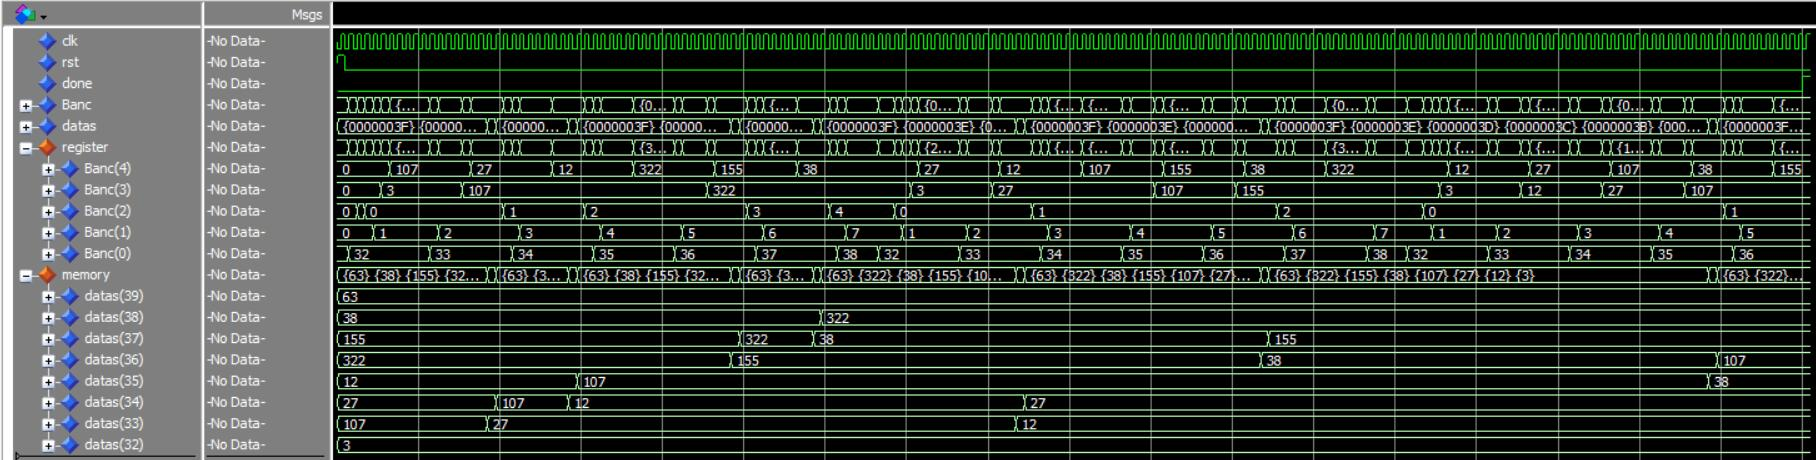
\includegraphics[width=1\textwidth]{picture/PUEXres.jpg}
    \caption{Simulation Waves of Processing Unit with IS Increasing}     
    \label{fig:PUEXres}
\end{figure}










%%%%%%%%%%%%%%%%%%%%%%%%%%%%%%%%%%%%%%%%%%%
\appendix

\section{Appendices}
\label{AppendicesA}

In Section \ref{sec:Assemble ALU and Register File}, the full view of the waves in simulation \textbf{Assemble\_ALU\_and\_Regist\_File\_tb.vhd} is shown as Figure \ref{fig:ModelSim_ assemble_processing_unit_tb(test_bench)}.

\begin{figure}[htp]
  \centering
  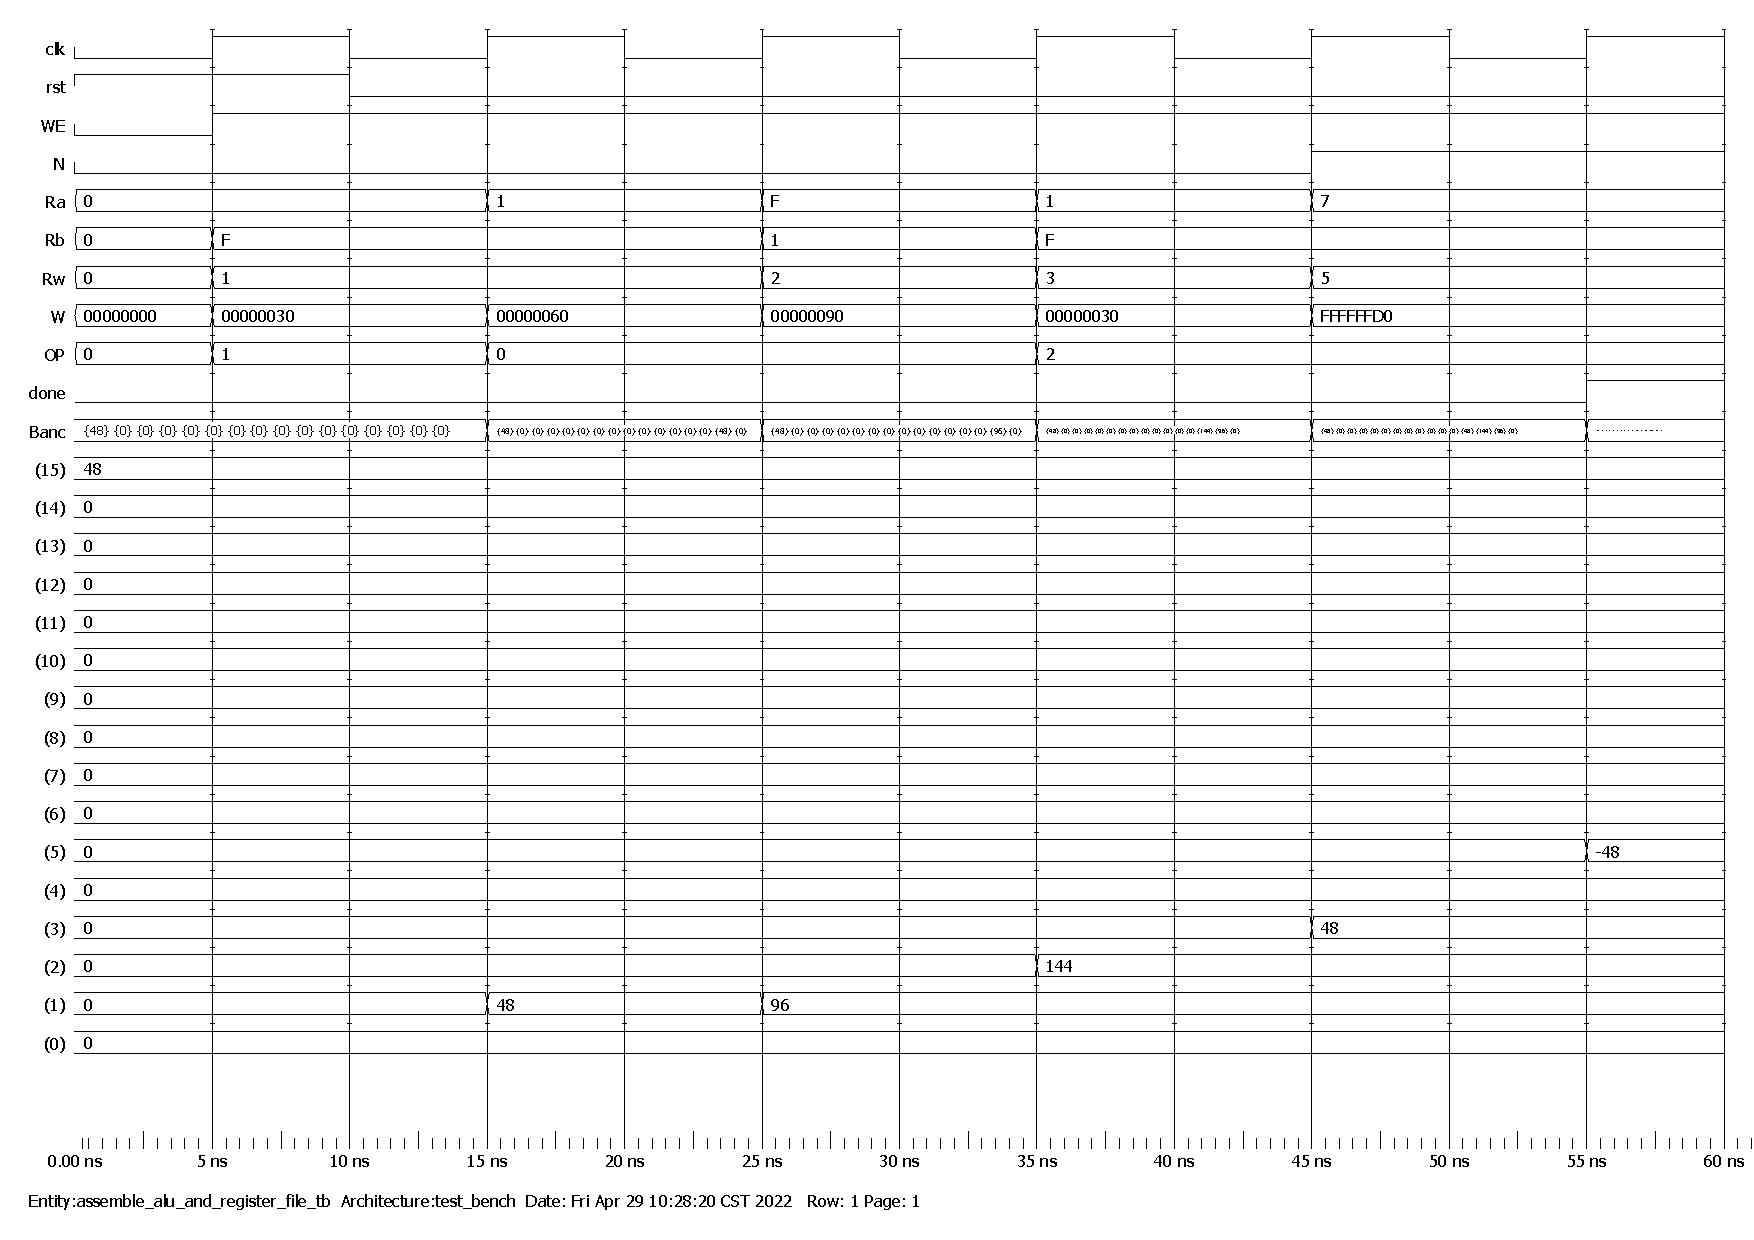
\includegraphics[width=1.5\textwidth,angle = 270]{picture/ModelSim_ assemble_processing_unit_tb(test_bench).pdf}
  \caption{Simulation Waves of Assemble ALU and Regist\_File}     
  \label{fig:ModelSim_ assemble_processing_unit_tb(test_bench)}
\end{figure}

In Section \ref{sec:Simulation for Instruction Management Unit}, the full view of the waves in simulation \textbf{Instruction\_Management\_Unit\_tb.vhd} is shown as Figure \ref{fig:ModelSim_ insmanagement_tb(bench)}.

\begin{figure}[htp]
  \centering
  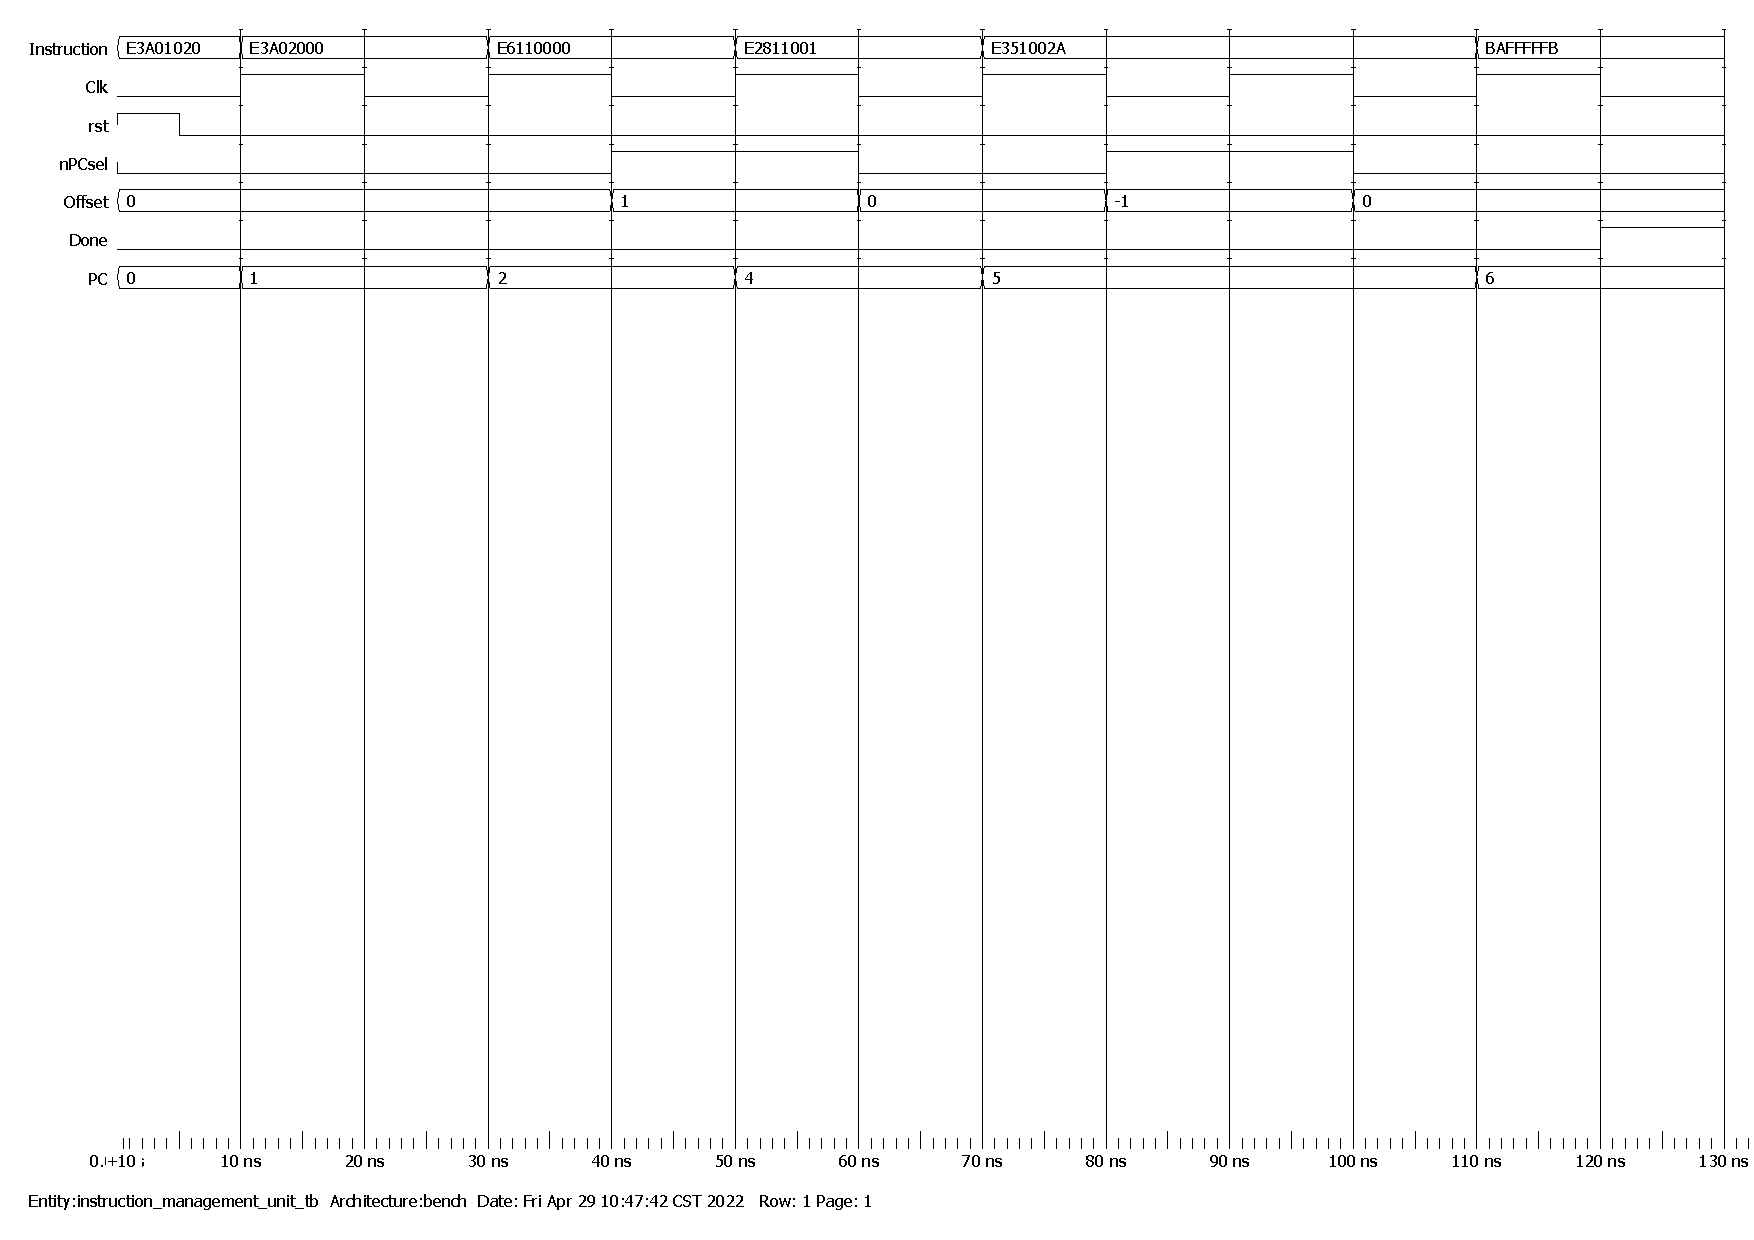
\includegraphics[width=1.5\textwidth, angle=270]{picture/ModelSim_ insmanagement_tb(bench).pdf}
  \caption{Simulation of Instruction Management Unit}     
  \label{fig:ModelSim_ insmanagement_tb(bench)}
\end{figure}

In Section \ref{sec:Instruction Decoder}, the ARM instruction set formats are shown as Figure \ref{fig:AISF}.

\begin{figure}[htp]
  \centering
  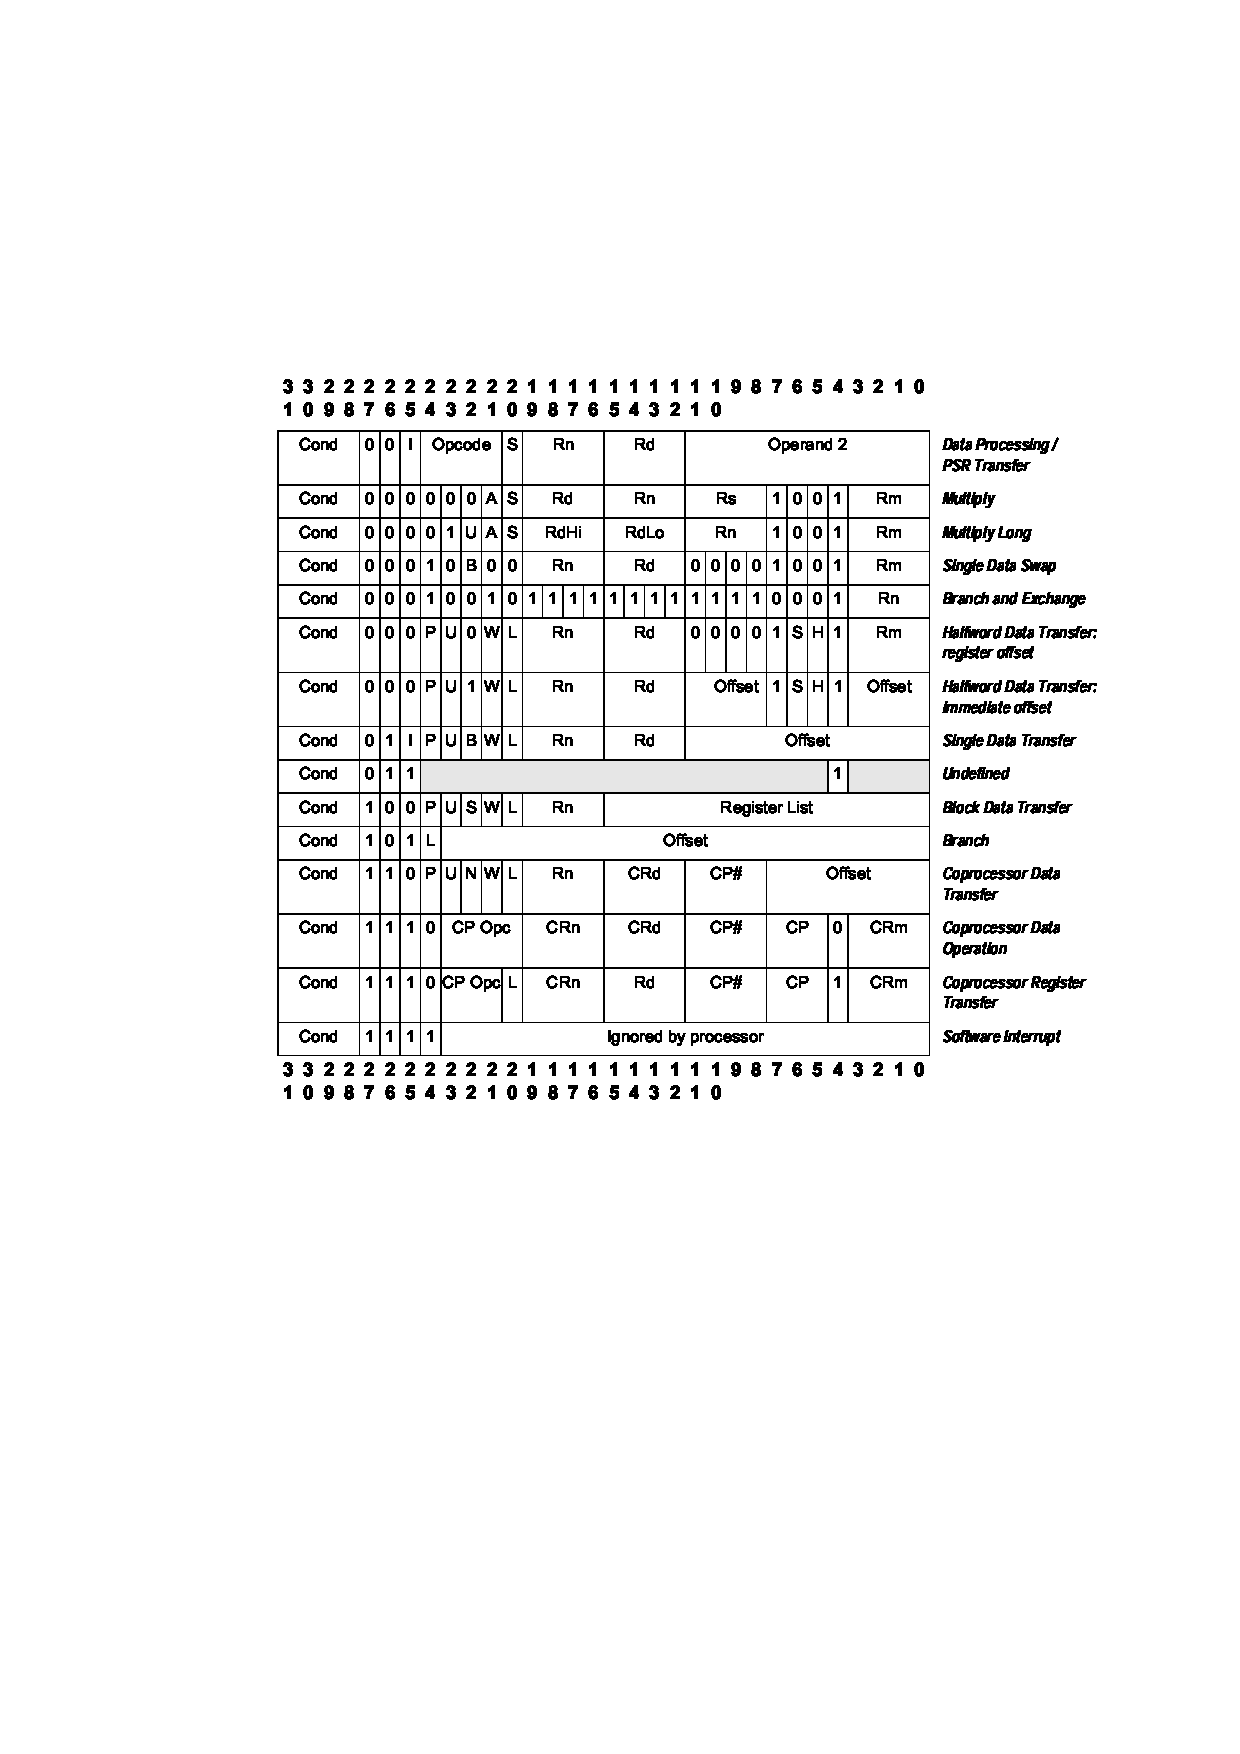
\includegraphics[width=1\textwidth]{picture/ARM instruction set formats.pdf}
  \caption{ARM Instruction Set Formats}     
  \label{fig:AISF}
\end{figure}

And in the same sectoin (Section \ref{sec:Instruction Decoder}), the detailed information about \texttt{Single Data Transfer} and \texttt{Branch}
are shown as Figure \ref{fig:Single data transfer instructions} and Figure \ref{fig:Branch instructions}.

\begin{figure}[htp]
  \centering
  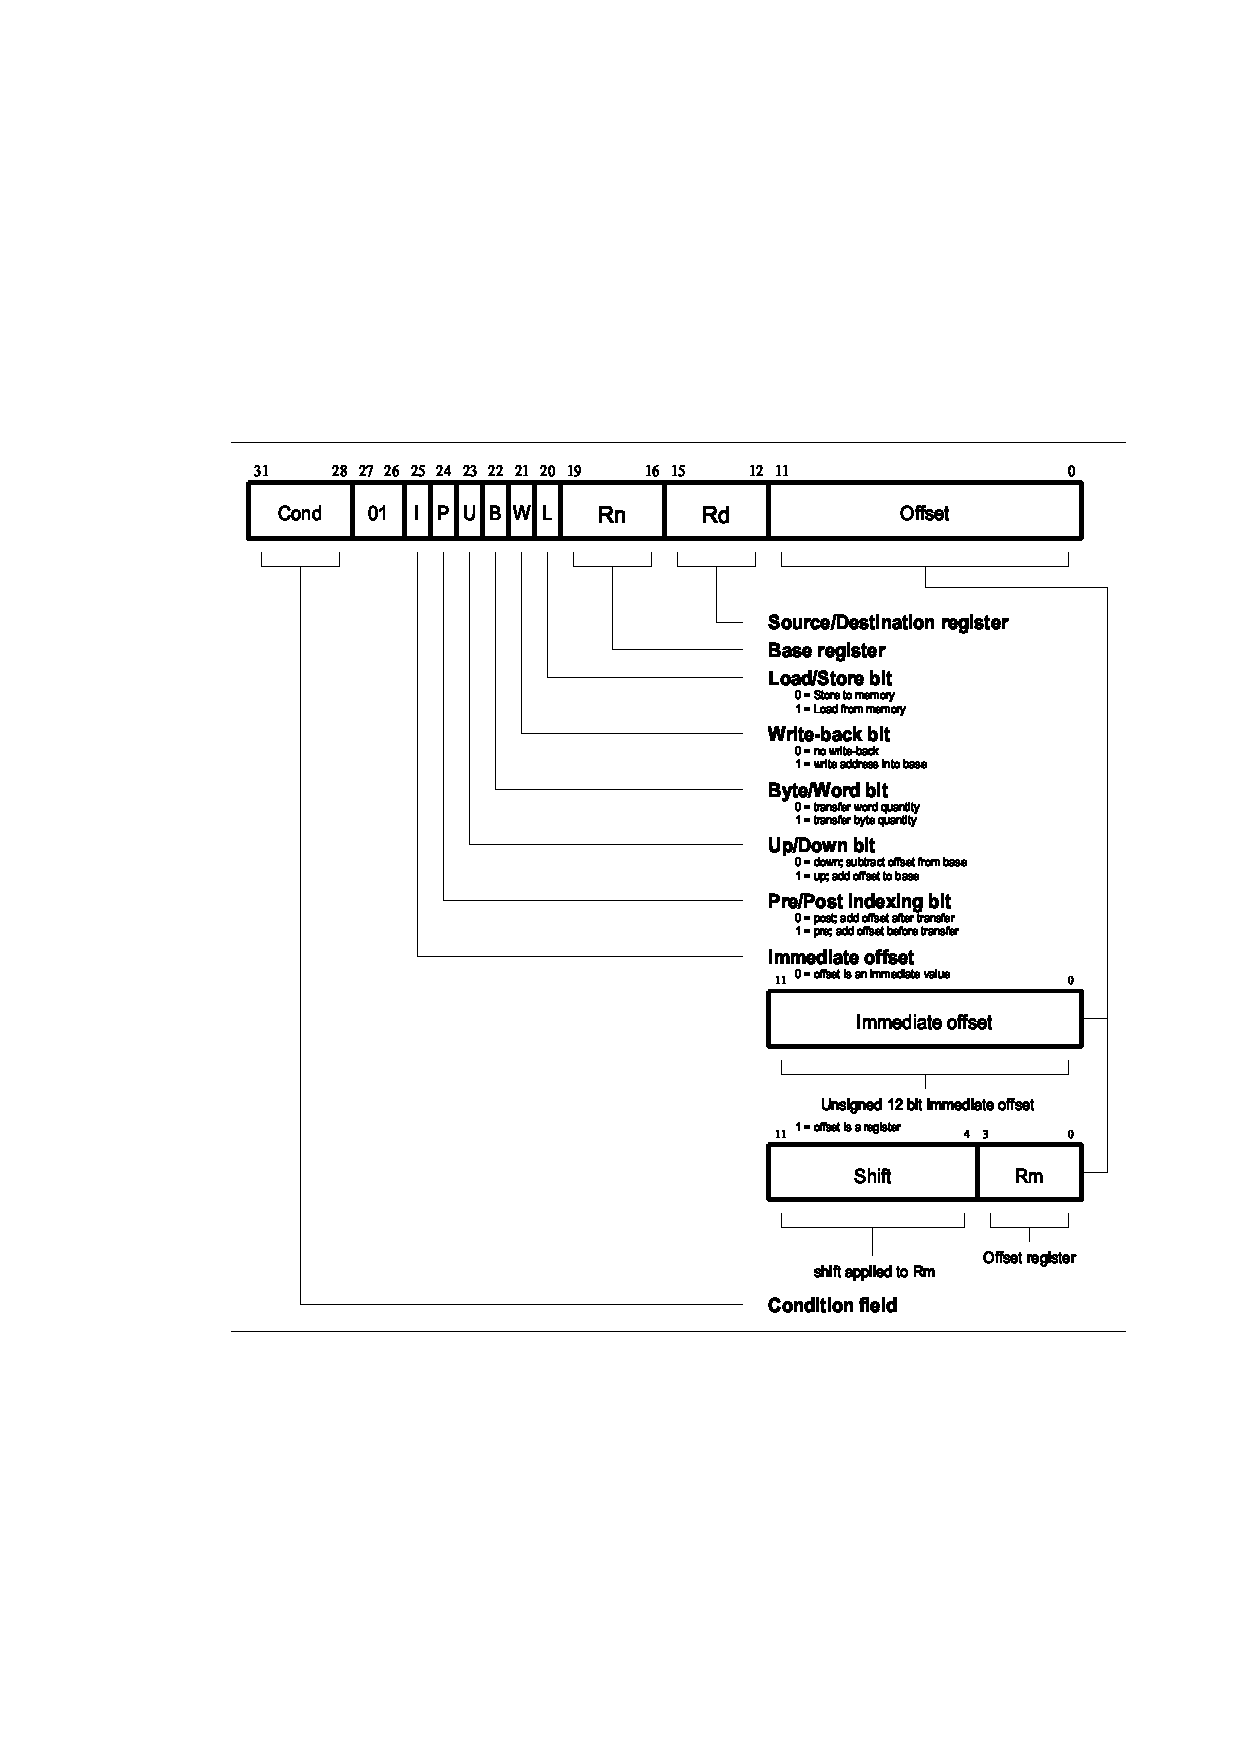
\includegraphics[width=1\textwidth]{picture/Single data transfer instructions.pdf}
  \caption{Single Data Transfer Instructions}     
  \label{fig:Single data transfer instructions}
\end{figure}

\begin{figure}[htp]
  \centering
  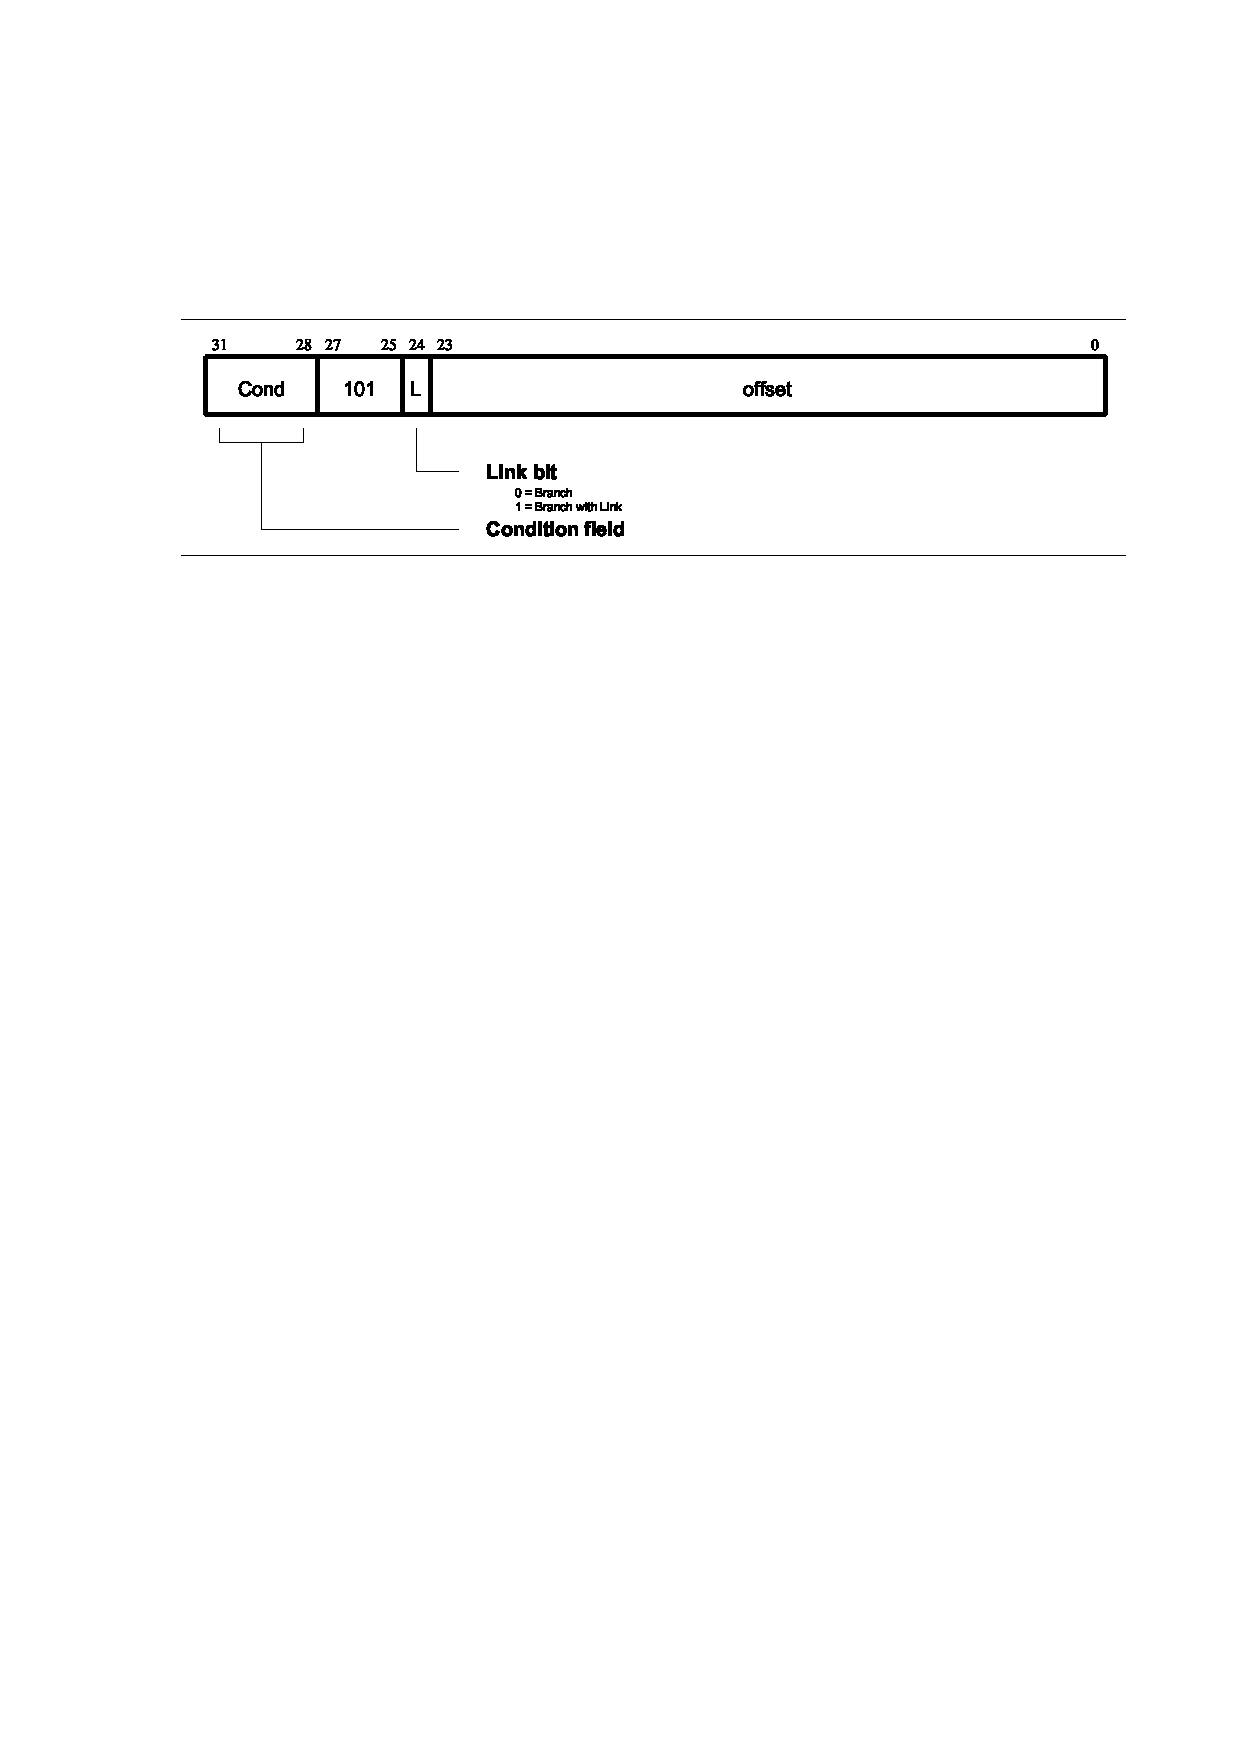
\includegraphics[width=1\textwidth]{picture/Branch instructions.pdf}
  \caption{Branch Instructions}     
  \label{fig:Branch instructions}
\end{figure}

In Section \ref{sec:Assemble Processor}, the Block Diagram of Processor as Figure \ref{fig:PU}.

\begin{figure}[htp]
  \centering
  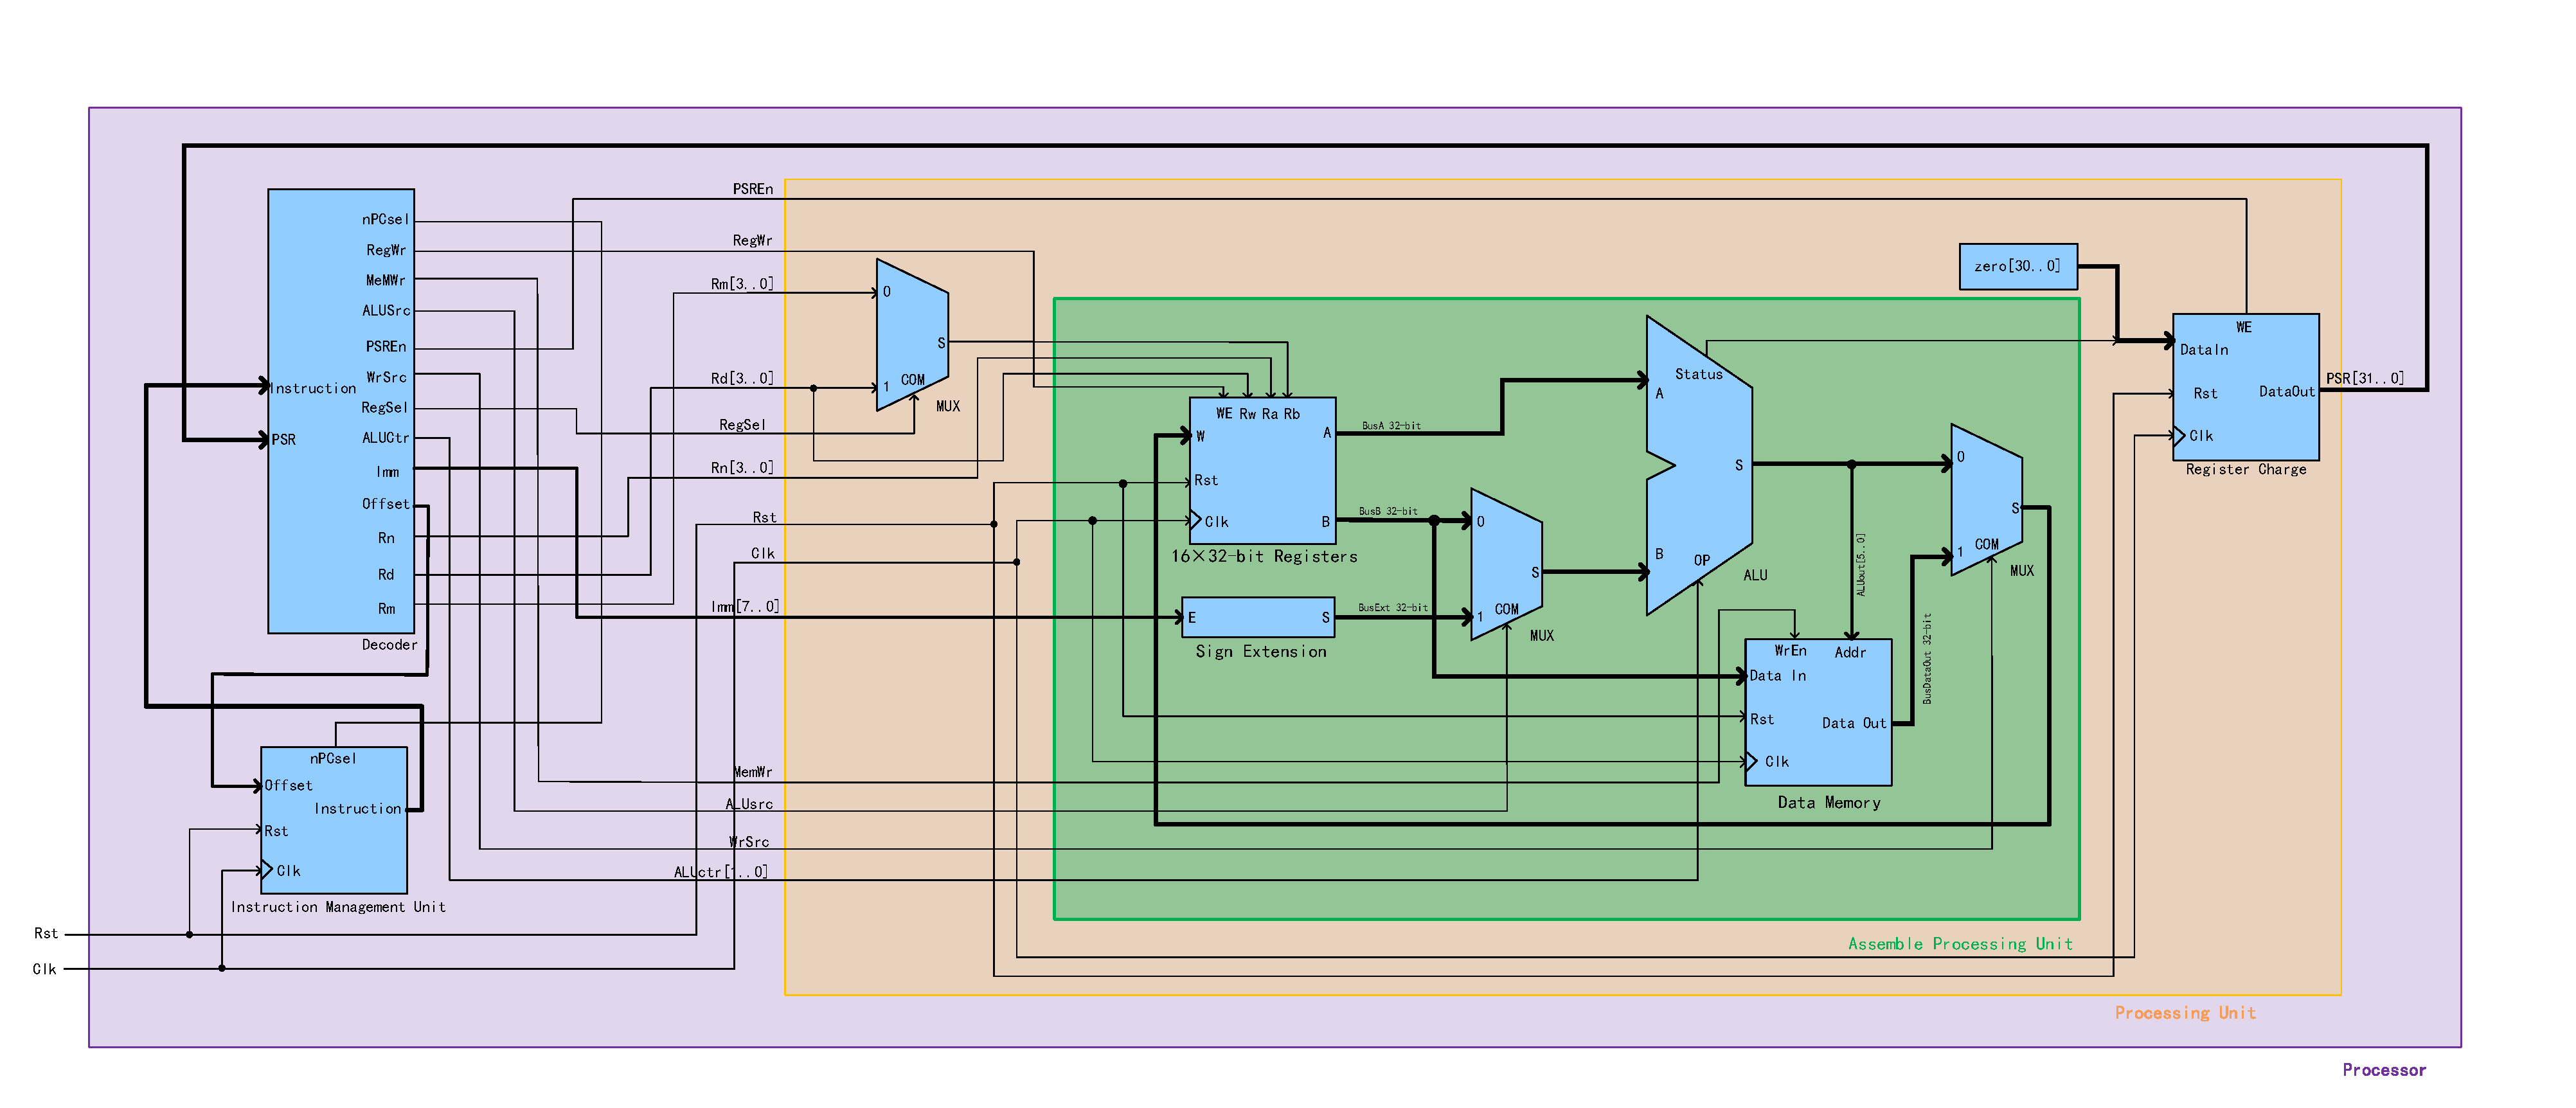
\includegraphics[width=1.5\textwidth, angle=270]{picture/PU.pdf}
  \caption{Processor Block Diagram}     
  \label{fig:PU}
\end{figure}

In Section \ref{sec:Simulate Processor}, 
the full view of the waves in simulation \textbf{Processor\_tb.vhd} in \textbf{part 4} is shown 
as Figure \ref{fig:ModelSim_ processeur_tb(bench)}.
\begin{figure}[htp]
  \centering
    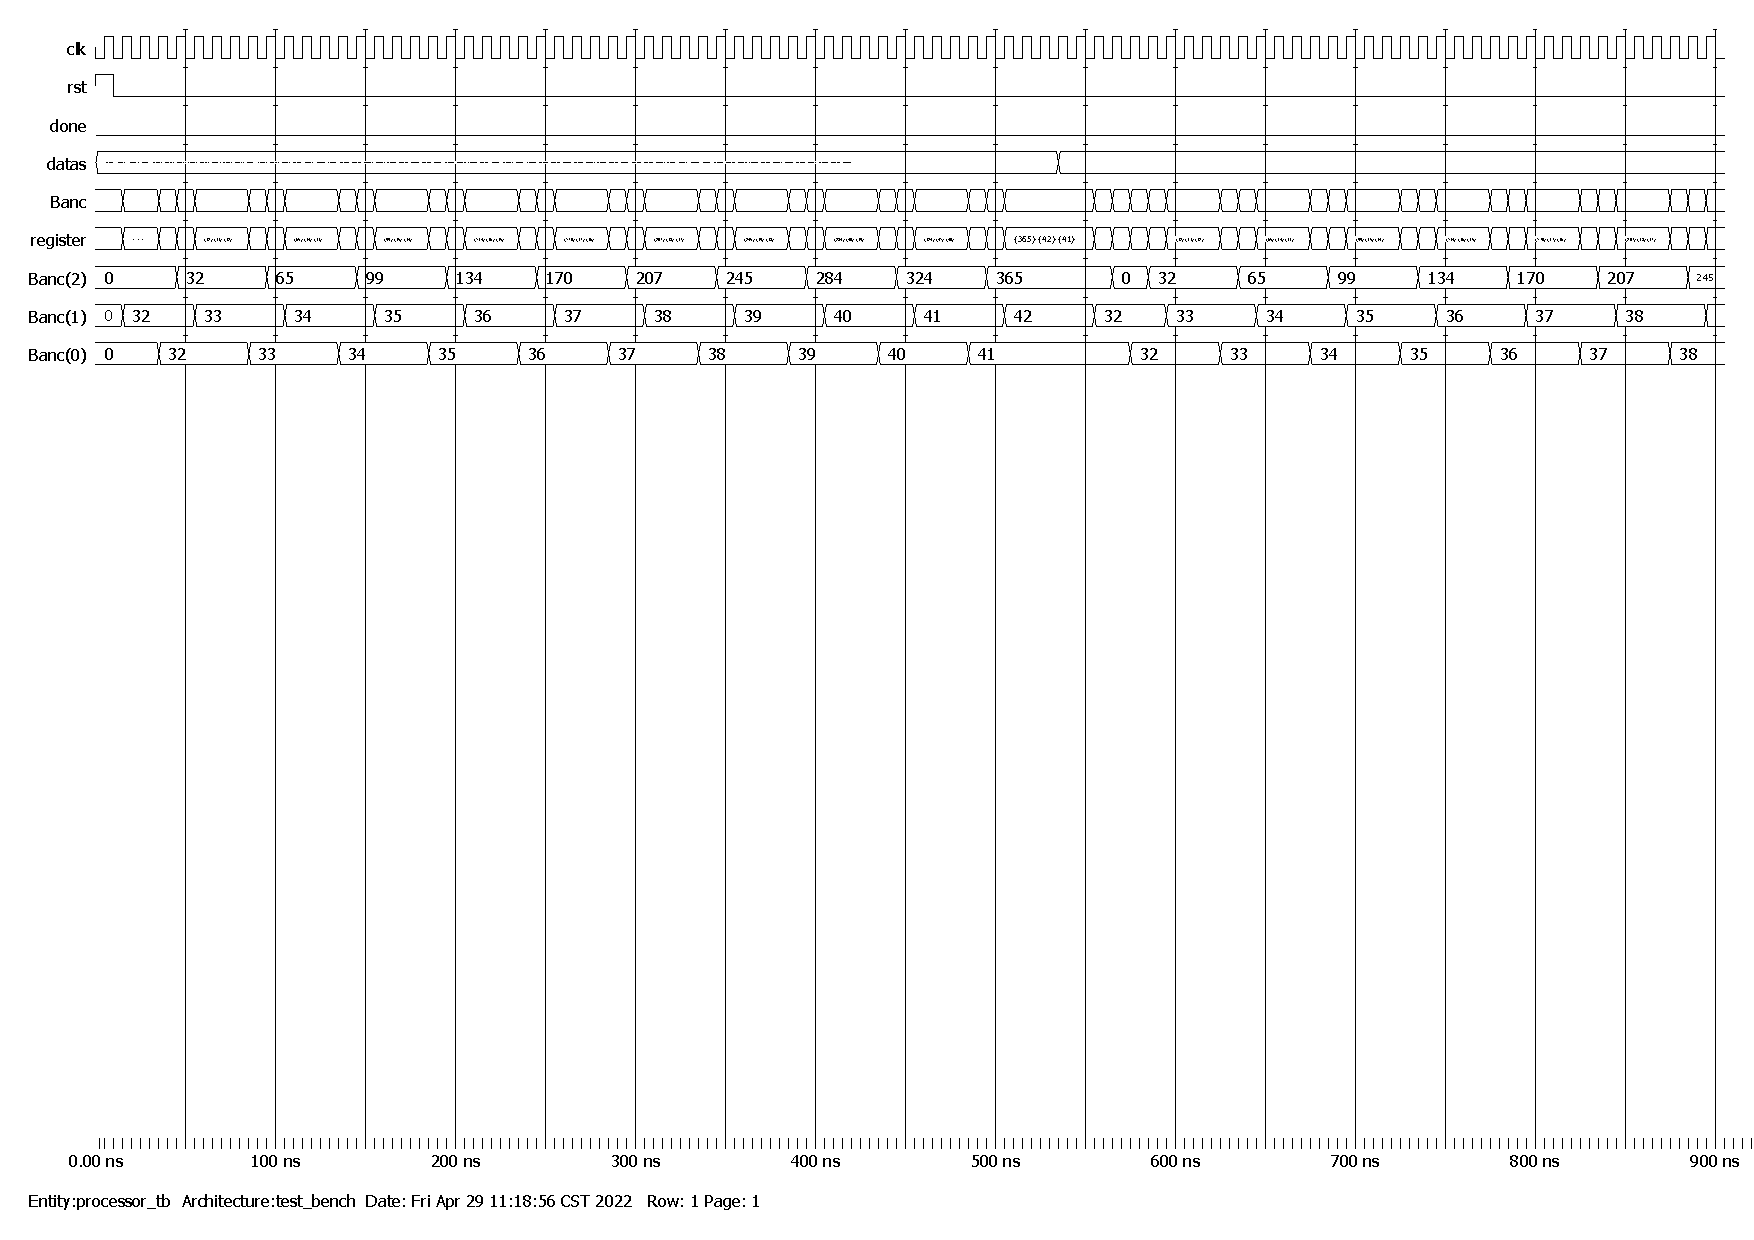
\includegraphics[width=1.5\textwidth,angle = 270]{picture/ModelSim_ processeur_tb(bench) 1.pdf}
\end{figure}

\begin{figure}[htp]
  \centering
    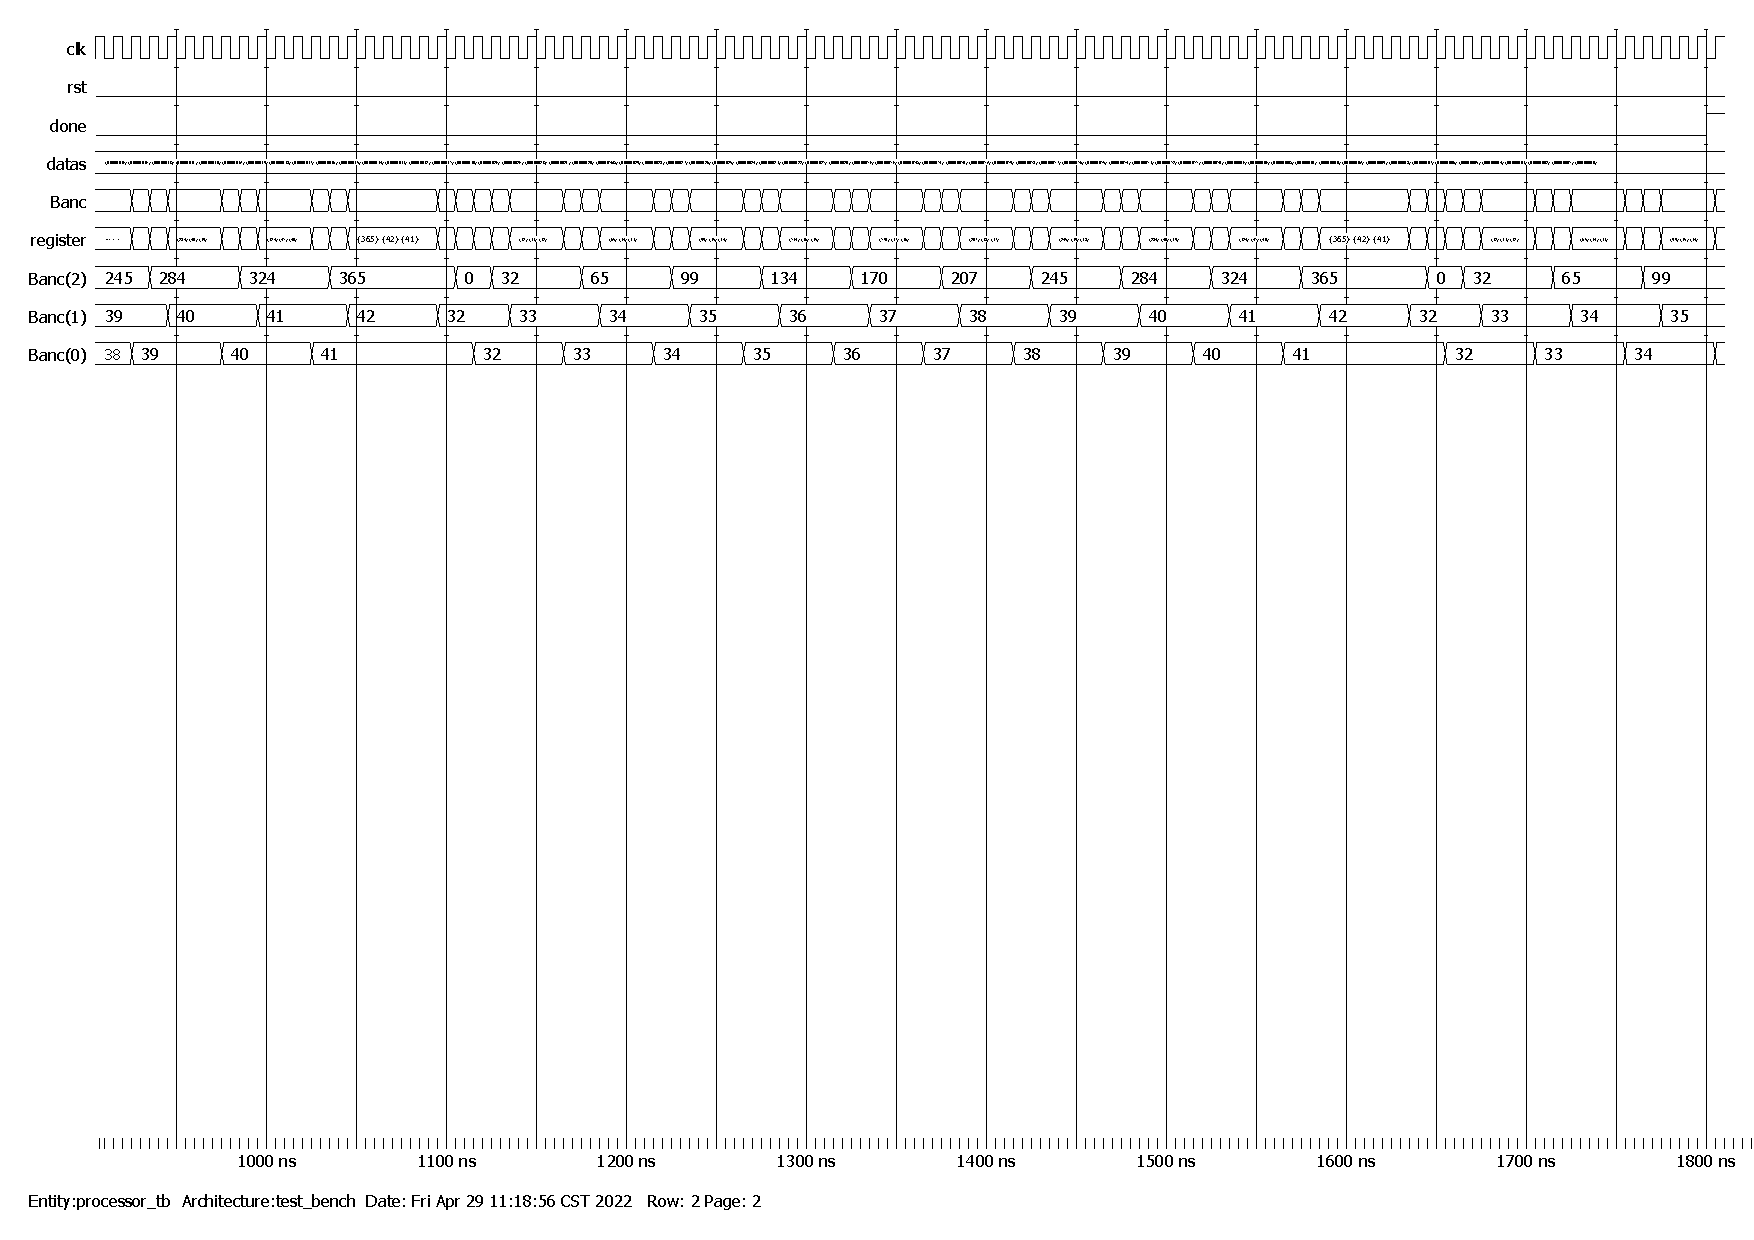
\includegraphics[width=1.5\textwidth,angle = 270]{picture/ModelSim_ processeur_tb(bench) 2.pdf}
    \caption{Simulation Waves of Processor in Part 4}  
  \label{fig:ModelSim_ processeur_tb(bench)}
\end{figure}

In Section \ref{sec:Test Processor Completely (Test Complet du Processeur)}, 
the full view of the waves in simulation in \textbf{part 5} is shown 
as Figure \ref{fig:ModelSim_ processeur_tb(bench) C}.
\begin{figure}[htp]
  \centering
    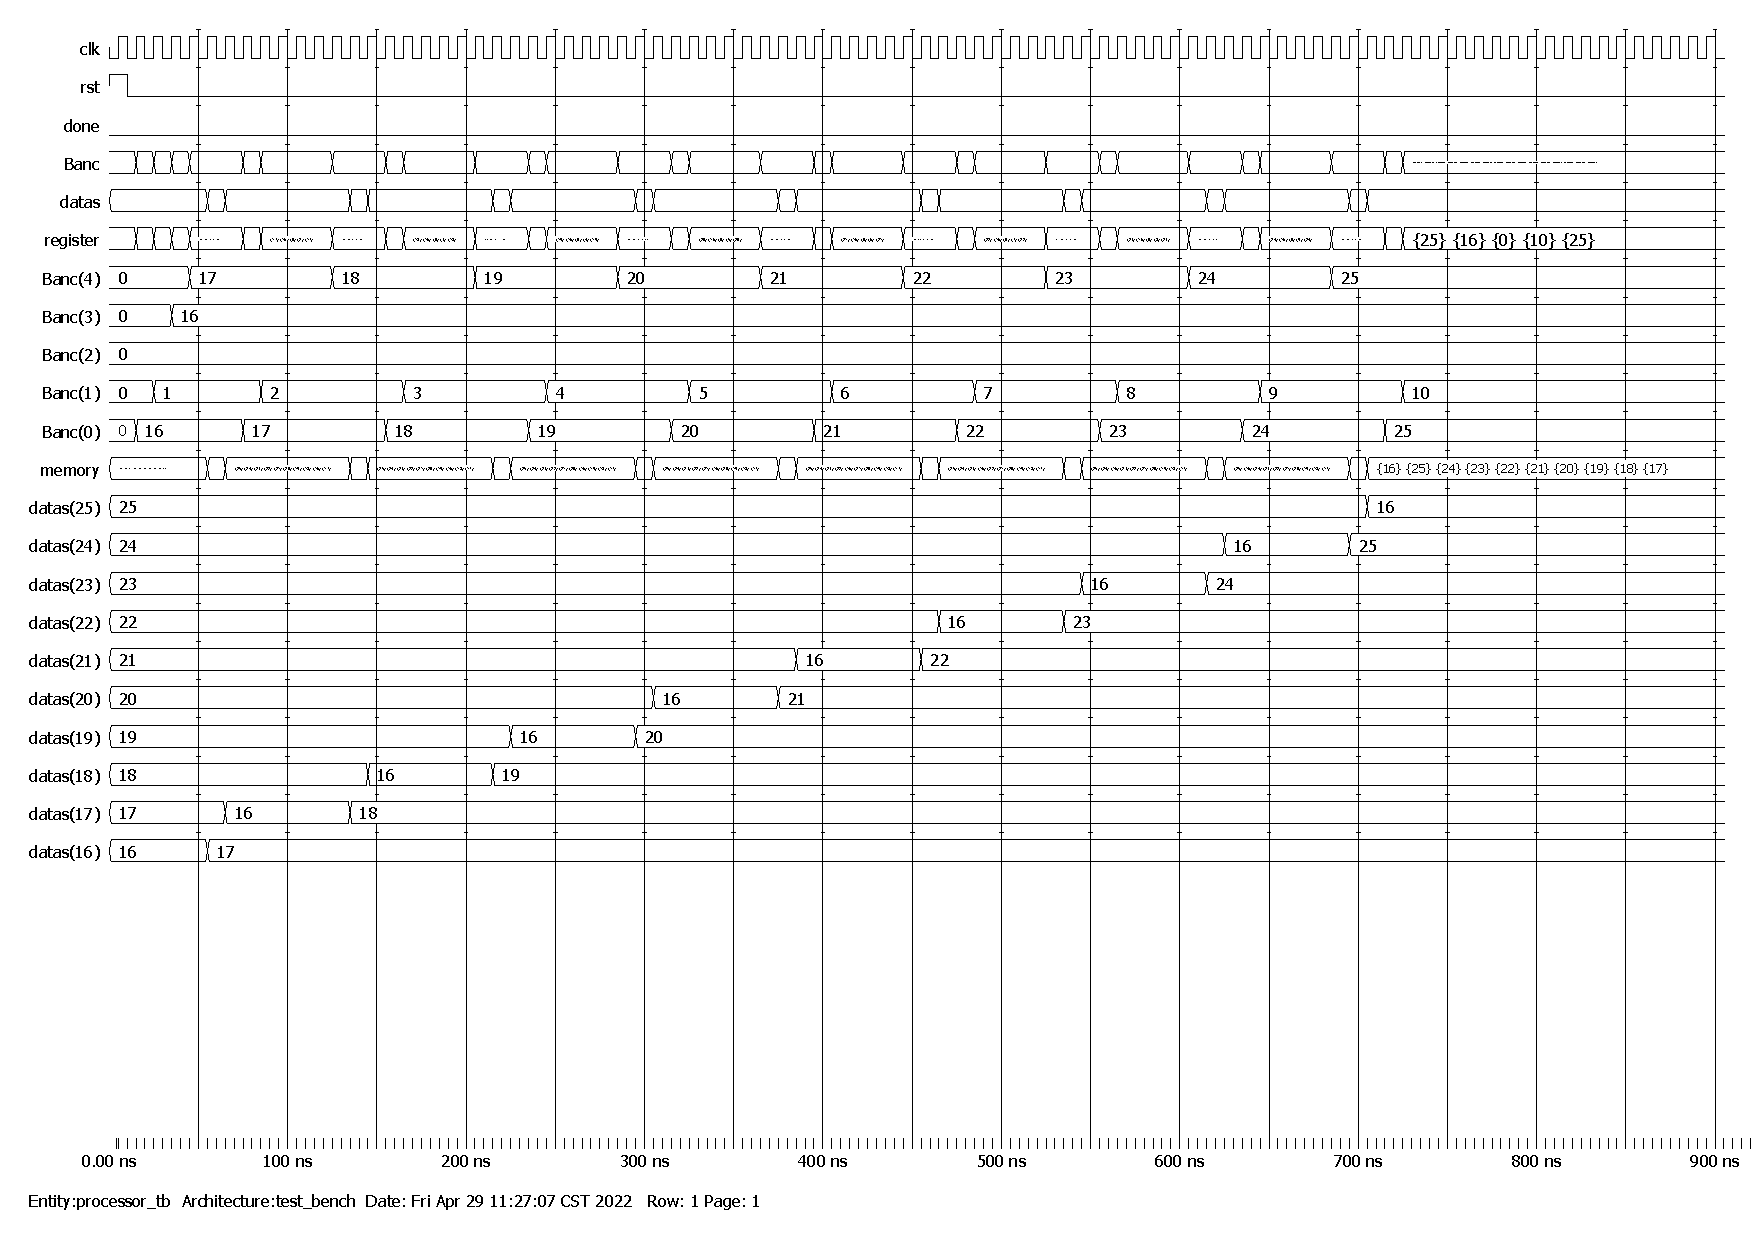
\includegraphics[width=1.5\textwidth,angle = 270]{picture/ModelSim_ processeur_tb(bench) C 1.pdf}
\end{figure}

\begin{figure}[htp]
  \centering
    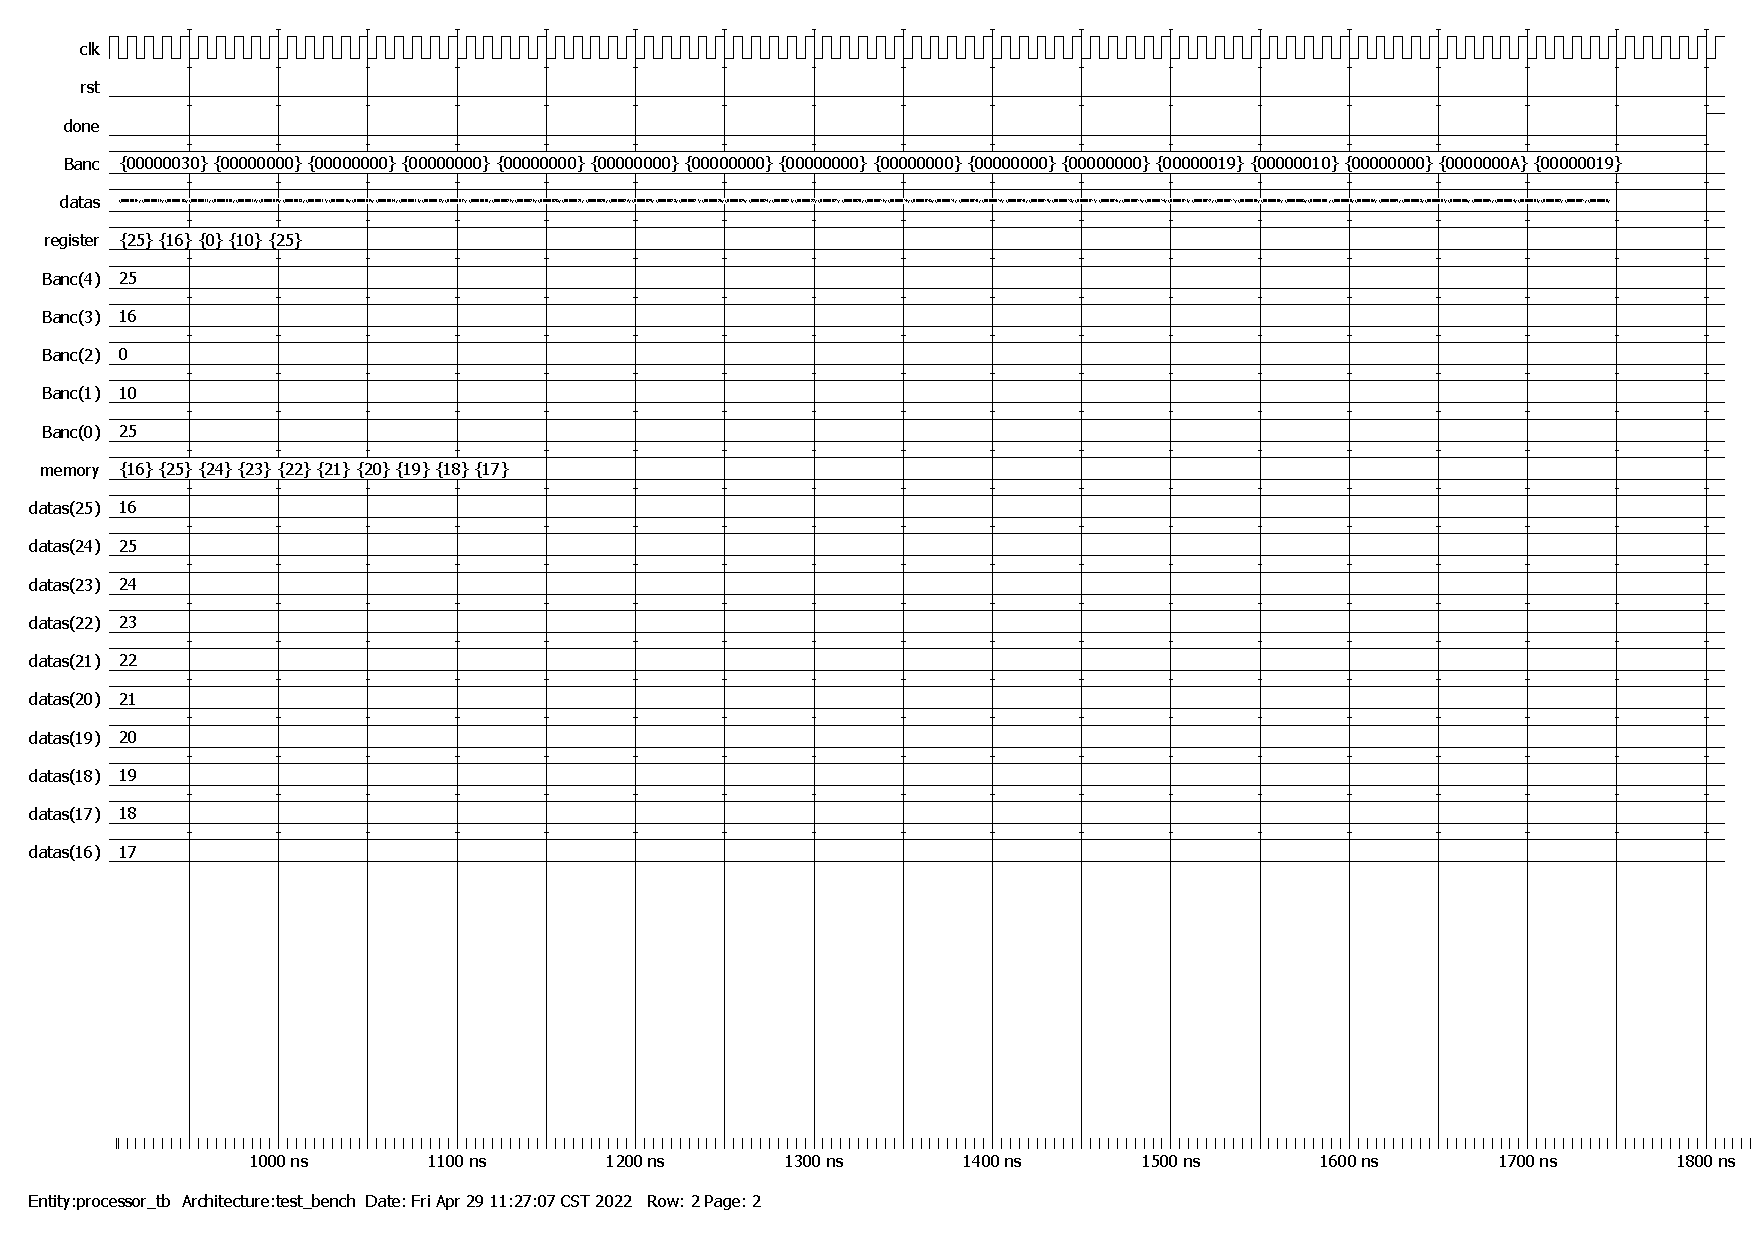
\includegraphics[width=1.5\textwidth,angle = 270]{picture/ModelSim_ processeur_tb(bench) C 2.pdf}
    \caption{Simulation Waves of Processor Completely in Part 5}  
  \label{fig:ModelSim_ processeur_tb(bench) C}
\end{figure}

In Section \ref{sec:Increasing the Instruction Set (Augmentation du Jeu d'Instruction)}, 
the full view of the waves in simulation in \textbf{part 6} is shown 
as Figure \ref{fig:ModelSim_ assemblage_tous_tb(test_bench)}.
\begin{figure}[htp]
  \centering
    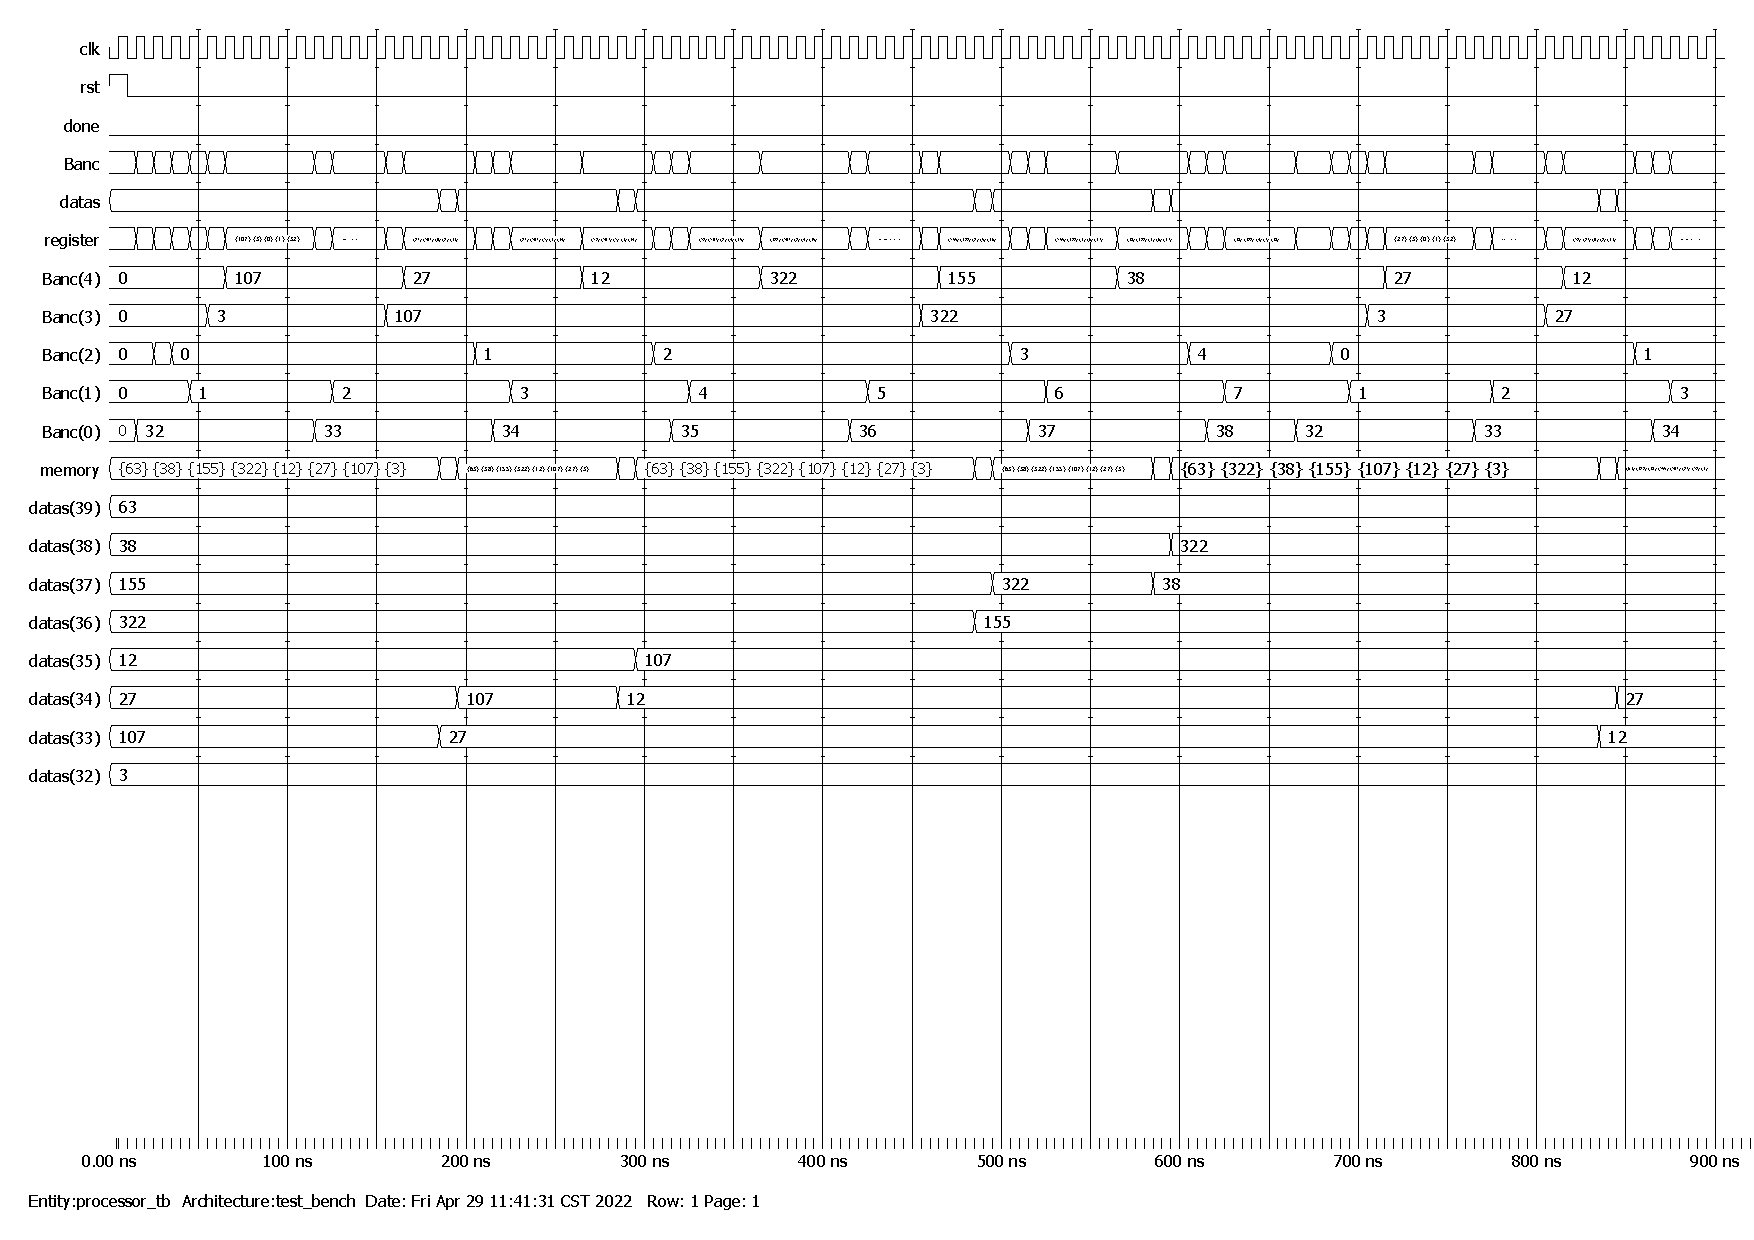
\includegraphics[width=1.5\textwidth,angle = 270]{picture/ModelSim_ assemblage_tous_tb(test_bench) 1.pdf}
\end{figure}

\begin{figure}[htp]
  \centering
    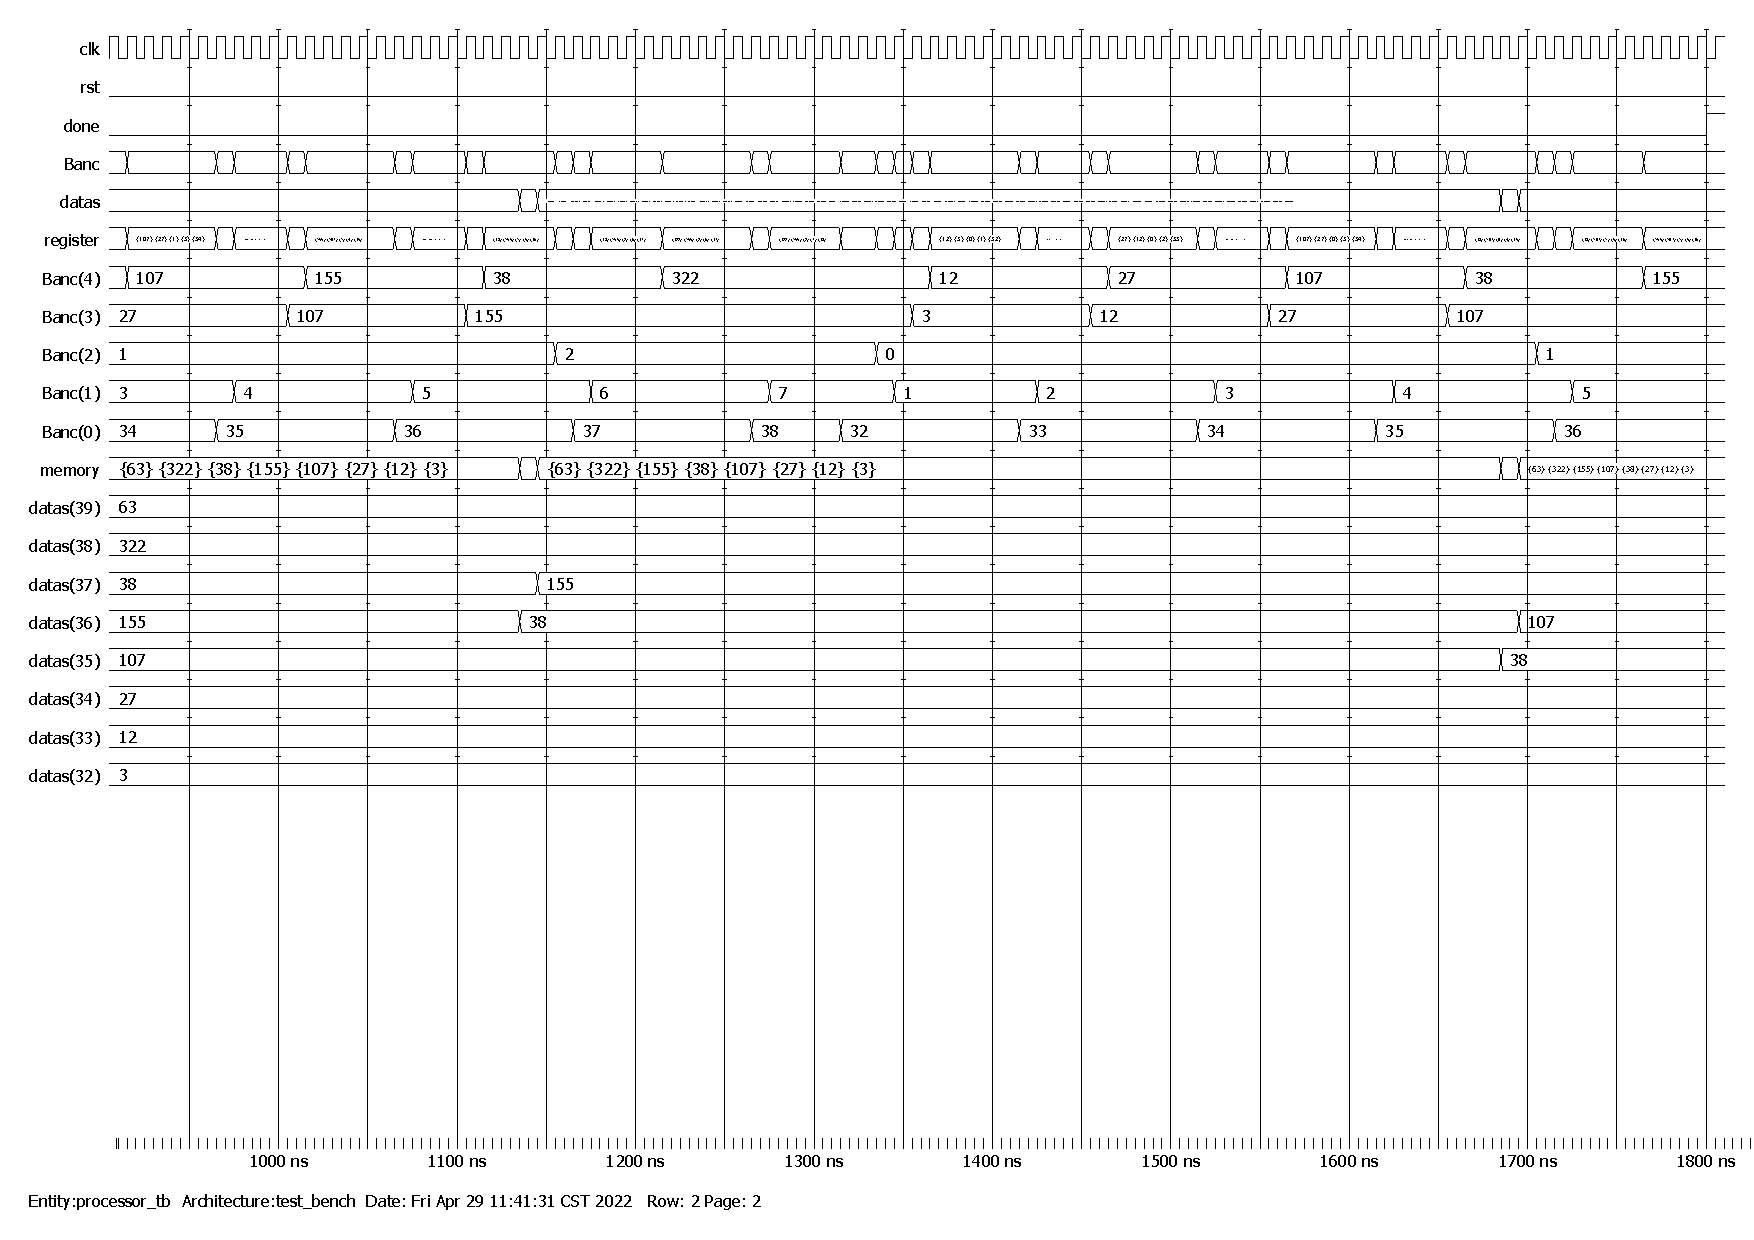
\includegraphics[width=1.5\textwidth,angle = 270]{picture/ModelSim_ assemblage_tous_tb(test_bench) 2.pdf}
    \caption{Simulation Waves of Processor with IS Increasing in Part 6}  
  \label{fig:ModelSim_ assemblage_tous_tb(test_bench)}
\end{figure}




%%%%%%%%%%%%%%%%%%%%%%%%%%%%%%%%%%%%%%%%%%%%%%
\clearpage
\bibliographystyle{plain}
\bibliography{bib_file}

\end{document}


 